% =============================================================
%  AFE control in the uvw frame: the five MATLAB Function blocks of afe_uvw_ctrl (pwr-control/library)
%  pwr-control documentation - compile with pdflatex (three times) from inside this folder:
%      pdflatex afe_uvw_ctrl.tex && pdflatex afe_uvw_ctrl.tex && pdflatex afe_uvw_ctrl.tex
%  Block diagrams are TikZ drawn in this file. The analytic figures (figures/res_pi_*.pdf) and the numbers of
%  Section 6 come from the companion script afe_uvw_ctrl_figures.py (numpy + matplotlib, no MATLAB):
%      python3 afe_uvw_ctrl_figures.py          -> figures/*.pdf, figures/afe_uvw_ctrl_numbers.txt
%  The two PNG figures of Section 9 are the output of the checks of the library package
%  (tools/check_afe_uvw_ctrl.py and test/afe_uvw_ctrl_test_loop.m of library/masked_models/afe_uvw_ctrl).
% =============================================================
\documentclass[11pt,a4paper]{scrartcl}
% ===================== PACKAGES =====================
\usepackage[british]{babel}
\usepackage[tmargin=1in, bmargin=1in, lmargin=0.75in, rmargin=0.75in]{geometry}
\usepackage[dvipsnames,table]{xcolor}  % prima di tikz, listings, ecc.

\usepackage{tikz}
\usepackage{graphicx}
\usepackage{pgfplots}
\pgfplotsset{width=12cm, compat=1.9}
\usepackage{setspace}
\usepackage{chemmacros}
\usepackage{chemfig}
\usepackage{esint}
\usepackage{tabularray}
\usepackage{makeidx}
\usepackage{epstopdf}
\usepackage{amssymb}
\usepackage{mathrsfs}
\usepackage{bm}
\usepackage{amsmath}
\usepackage{enumitem}
\usepackage[english]{varioref}
\usepackage{lipsum}
\usepackage{fancyhdr}
\usepackage{float}
\usepackage{empheq}
\usepackage[framemethod=tikz]{mdframed}
\numberwithin{equation}{section}
\usepackage{eso-pic}
\usepackage{calc}
\usepackage{nccmath}
\usepackage{caption}
\usepackage{subcaption}
\usepackage{gensymb}
\usepackage{amsfonts, amsthm, epsfig, epstopdf, titling, url, array}
\usepackage{tabularx}
\usepackage{makecell}
\usepackage{booktabs}
\usepackage{array}
\usepackage{siunitx}
\sisetup{input-digits=0123456789\pi}
\usepackage[symbol]{footmisc}
\usepackage{multicol}
\usepackage{boondox-cal}
\usepackage{blindtext}
\usepackage{changepage}
\usepackage{nomencl}
\usepackage{hyperref}
\usepackage{xurl}
\usepackage{ragged2e}
\usepackage[version=4]{mhchem}  % ← conflitto di opzioni
\usepackage{longtable}
\usepackage{chemformula}
\usetikzlibrary{arrows.meta,positioning,calc}

% ===================== SI UNITS =====================
\DeclareSIUnit\atm{atm}
\DeclareSIUnit{\var}{var}
\DeclareSIUnit{\pu}{p.u.}


% ===================== MATH OPERATORS =====================
\DeclareMathOperator{\rank}{rank}
\DeclareMathOperator{\atantwo}{atan2}
\DeclareMathOperator{\spn}{span}

% ===================== COMMANDS =====================
\newcommand{\abs}[1]{\left|#1\right|}
\newcommand{\sign}{\text{sign}}
\newcommand{\centered}[1]{\begin{tabular}{@{}l@{}} #1 \end{tabular}}

% ===================== COLORS =====================
\definecolor{mycolor1}{rgb}{0.97, 0.97, 0.97}
\definecolor{mycolor2}{rgb}{0.97, 0.97, 0.97}
\definecolor{tableShade}{gray}{0.9}

% ===================== THEOREM ENVIRONMENTS =====================
\theoremstyle{it}
\newtheorem{defn}{Definition}[section]
\newtheorem{assumption}{Assumption}[section]
\newtheorem{thm}{Theorem}[section]
\newtheorem{lemma}{Lemma}[section]
\newtheorem{corollary}{Corollary}[section]
\theoremstyle{definition}
\newtheorem{example}{Example}[section]

% ===================== CUSTOM ENVIRONMENTS =====================
\newenvironment{myitemize_1}{
	\begin{itemize}[topsep=0pt]
		\setlength{\topsep}{2pt}
		\setlength{\itemsep}{2pt}
		\setlength{\parskip}{2pt}
		\setlength{\parsep}{2pt}
	}{\end{itemize}}

\newmdenv[
innerlinewidth=0.5pt,
roundcorner=4pt,
backgroundcolor=mycolor2,
linecolor=mycolor1,
innerleftmargin=6pt,
innerrightmargin=6pt,
innertopmargin=6pt,
innerbottommargin=6pt
]{mybox}

% ===================== TABLE COLUMN TYPES =====================
\newcolumntype{Y}{>{\hsize=2\hsize}X}
\newcolumntype{Z}{>{\centering\arraybackslash\hsize=0.857\hsize}X}

% ===================== SECTION DEPTH =====================
\setcounter{secnumdepth}{3}
\setcounter{tocdepth}{3}

% ===================== PAGE STYLE =====================
\setlength{\headheight}{20pt}
\setlength{\headsep}{20pt}

\pagestyle{fancy}
\fancypagestyle{firstpage}{\rhead{}}
\fancyhead[L]{\slshape\nouppercase{\leftmark}}
\chead{}
\rhead{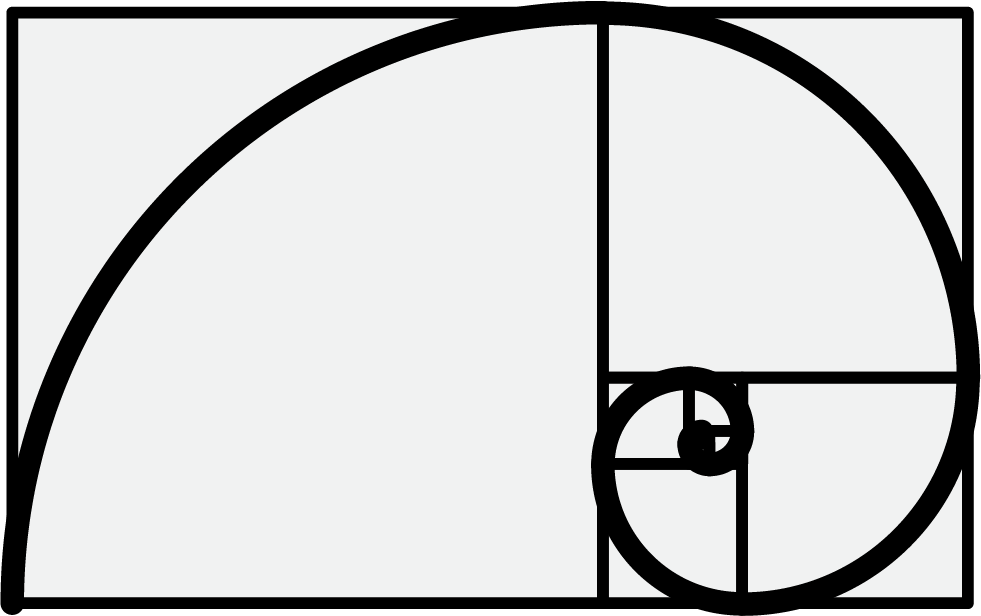
\includegraphics[height=0.75cm]{../../AAA_template_latex_settings/pwr-control_logo_doc.png}}
\lfoot{\href{http://www.pwr-control.com}{pwr-control.com}}
\cfoot{-\ \thepage\ -}
\rfoot{\textit{}}
\renewcommand{\headrulewidth}{0.4pt}
\renewcommand{\footrulewidth}{0.4pt}


\geometry{
	a4paper,
	top    = 2.5cm,
	bottom = 3.0cm,
	left   = 2.5cm,
	right  = 2.5cm
}

\hypersetup{
	colorlinks = true,
	urlcolor   = blue,
	linkcolor  = black,
	citecolor  = black
}

\pagenumbering{gobble}

\usetikzlibrary{shapes.geometric,fit,decorations.pathreplacing}

\newcommand{\ped}[1]{_{\mathrm{#1}}}
\newcommand{\code}[1]{\texttt{#1}}
\newcommand{\sat}{\operatorname{sat}}
\renewcommand{\tabularxcolumn}[1]{>{\raggedright\arraybackslash}p{#1}}
\setlength{\emergencystretch}{3em}
\sisetup{per-mode=symbol}

% ---------------- document metadata (read by the title page) ----------------
\newcommand{\DocCategory}{Technical Note}
\newcommand{\DocField}{Power Electronics and Control Systems}

\newcommand{\DocTitle}{%
	{\fontsize{20}{24}\selectfont\bfseries AFE control in the uvw frame} \\[16pt]
	{\fontsize{16}{20}\selectfont\bfseries the five MATLAB Function blocks of \code{afe\_uvw\_ctrl}: sequences, fault ride-through, reactive current loops, per-phase resonant PI and islanding detection}
}

\newcommand{\DocSubtitle}{%
	The controller of the model \code{afe\_uvw\_three\_phase} as it is written in the library package \code{masked\_models/afe\_uvw\_ctrl} of \code{pwr-control/library}: the algorithm of each block, equation by equation, with the discrete implementation of the resonant PI current controller and what it means for the poles of the loop.
}

\newcommand{\DocAuthor}{Davide Bagnara}
\newcommand{\DocRevision}{00}
\newcommand{\DocDate}{November 2026}

\newcommand{\DocAbstract}{%
	The control of the three-phase active front end (AFE) of the model \code{afe\_uvw\_three\_phase} works in the stationary frame: one resonant PI per phase makes the converter current follow a sinusoidal reference, while the slow loops (reactive current of the positive and the negative sequence, fault ride-through) work on moving averages of the grid quantities in the positive and the negative synchronous frame. The library package \code{afe\_uvw\_ctrl} rewrites this control as five MATLAB Function blocks with one parameter structure. This note describes the algorithms as they are in the code: the Clarke and sequence transformations and the moving average with a fractional window, the voltage-rate observers and the state machine of the fault ride-through with the reactive current references of VDE-AR-N 4110, the three clamped PIs of the reactive current loops, the per-phase resonant PI with its forward Euler discretization, the vector limiter, the output delay and the zero-sequence loop, and the new passive islanding detector. The resonant PI is analysed in detail: with the damping of the model ($\delta = 0.015$) the forward Euler resonator has its poles just outside the unit circle ($|z| = 1.000182$), so the controller alone is marginally unstable and its gain at \SI{50}{\hertz} is 11.4 instead of the 4.3 of the continuous design; the current loop with the plant is stable (phase margin \ang{69}, sensitivity \SI{-41}{\decibel} at \SI{50}{\hertz}). The parameter structure, the mapping to the model init, the checks against the original block diagrams and the open points close the note.
}

\newcommand{\RevisionHistory}{%
	00 & November 2026 & First issue: the five blocks of \code{afe\_uvw\_ctrl} (library PR \#35), resonant PI analysis, parameters, checks, open points. & \DocAuthor \\
}

\newcommand{\MetaLabelA}{Project Repository}
\newcommand{\MetaValueAUrl}{https://github.com/pwr-control/library.git}
\newcommand{\MetaValueALabel}{library.git (masked\_models/afe\_uvw\_ctrl)}

\newcommand{\MetaLabelB}{Framework}
\newcommand{\MetaValueB}{MATLAB/Simulink, GNU Octave, Python}

\begin{document}

% =============================================================
%  pwr-control LaTeX template - FRONTESPIZIO
%
%  Da richiamare come prima istruzione dopo \begin{document}:
%      % =============================================================
%  pwr-control LaTeX template - FRONTESPIZIO
%
%  Da richiamare come prima istruzione dopo \begin{document}:
%      % =============================================================
%  pwr-control LaTeX template - FRONTESPIZIO
%
%  Da richiamare come prima istruzione dopo \begin{document}:
%      \input{../../AAA_template_latex_settings/titlepage}
%
%  Il documento deve definire prima di \begin{document}:
%      \DocCategory   categoria del documento
%      \DocField      area tecnica
%      \DocTitle      titolo (una o due righe)
%      \DocSubtitle   sottotitolo
%      \DocAuthor     autore/i, separati da virgola
%      \DocRevision   numero di revisione corrente (es. 00)
%      \DocDate       data della revisione corrente
%      \DocAbstract   abstract
%      \RevisionHistory  righe della tabella di revisione, nel formato
%                        Rev. & Date & Description & Authors \\
%      \MetaLabelA \MetaValueAUrl \MetaValueALabel
%      \MetaLabelB \MetaValueB
% =============================================================

\providecommand{\DocCategory}{Technical Research Report}
\providecommand{\DocField}{Power Electronics and Control Systems}
\providecommand{\DocSubtitle}{}
\providecommand{\DocRevision}{00}
\providecommand{\DocAbstract}{}
\providecommand{\RevisionHistory}{%
	\DocRevision & \DocDate & First issue. & \DocAuthor \\
}

\titlepage

% ---- Intestazione centrata ----
\begin{center}
	{\Large\scshape \DocCategory}\\[8pt]
	{\large\scshape \DocField}
\end{center}

\vspace{30pt plus 4pt minus 14pt}
\noindent\rule{\linewidth}{0.8pt}

% ---- Titolo ----
\begin{center}
	\DocTitle
\end{center}

\vspace{4pt}
\noindent\rule{\linewidth}{2.2pt}

% ---- Sottotitolo ----
\begin{center}
	\begin{onehalfspace}
		{\large\itshape \DocSubtitle}
	\end{onehalfspace}
\end{center}

% ---- Authors / Revision / Date ----
\vspace{30pt plus 4pt minus 14pt}

\noindent
\begin{minipage}[t]{0.46\linewidth}
	\raggedright
	\textbf{Authors:}\\[2pt]
	\DocAuthor
\end{minipage}%
\hfill
\begin{minipage}[t]{0.22\linewidth}
	\centering
	\textbf{Revision:}\\[2pt]
	\DocRevision
\end{minipage}%
\hfill
\begin{minipage}[t]{0.30\linewidth}
	\raggedleft
	\textbf{Date:}\\[2pt]
	\DocDate
\end{minipage}

\vspace{10pt}
\noindent\rule{\linewidth}{0.8pt}

% ---- Abstract ----
\vspace{24pt plus 4pt minus 12pt}

\begin{center}
	\begin{minipage}{0.88\linewidth}
		\footnotesize
		\begin{onehalfspace}
			\textbf{Abstract:} \DocAbstract
		\end{onehalfspace}
	\end{minipage}
\end{center}

\vfill

% ---- Revision history ----
\begin{center}
	\begin{minipage}{0.96\linewidth}
		\centering
		{\footnotesize\scshape Revision history}\\[6pt]
		{\footnotesize
			\begin{tabular}{@{}cl>{\raggedright\arraybackslash}p{0.36\linewidth}>{\raggedright\arraybackslash}p{0.28\linewidth}@{}}
				\toprule
				\textbf{Rev.} & \textbf{Date} & \textbf{Description} & \textbf{Authors} \\
				\midrule
				\RevisionHistory
				\bottomrule
			\end{tabular}}
	\end{minipage}
\end{center}

\vspace{18pt plus 4pt minus 10pt}

% ---- Metadati in fondo ----
\noindent
\begin{tabular}{@{} r @{\quad} l @{}}
	\textsc{\MetaLabelA:} & {\href{\MetaValueAUrl}{\MetaValueALabel}} \\[3pt]
	\textsc{\MetaLabelB:} & {\MetaValueB}       \\[3pt]
\end{tabular}

% =============================================================
%  Fine frontespizio
% =============================================================
\newpage
\pagenumbering{arabic}
\setcounter{page}{1}

%
%  Il documento deve definire prima di \begin{document}:
%      \DocCategory   categoria del documento
%      \DocField      area tecnica
%      \DocTitle      titolo (una o due righe)
%      \DocSubtitle   sottotitolo
%      \DocAuthor     autore/i, separati da virgola
%      \DocRevision   numero di revisione corrente (es. 00)
%      \DocDate       data della revisione corrente
%      \DocAbstract   abstract
%      \RevisionHistory  righe della tabella di revisione, nel formato
%                        Rev. & Date & Description & Authors \\
%      \MetaLabelA \MetaValueAUrl \MetaValueALabel
%      \MetaLabelB \MetaValueB
% =============================================================

\providecommand{\DocCategory}{Technical Research Report}
\providecommand{\DocField}{Power Electronics and Control Systems}
\providecommand{\DocSubtitle}{}
\providecommand{\DocRevision}{00}
\providecommand{\DocAbstract}{}
\providecommand{\RevisionHistory}{%
	\DocRevision & \DocDate & First issue. & \DocAuthor \\
}

\titlepage

% ---- Intestazione centrata ----
\begin{center}
	{\Large\scshape \DocCategory}\\[8pt]
	{\large\scshape \DocField}
\end{center}

\vspace{30pt plus 4pt minus 14pt}
\noindent\rule{\linewidth}{0.8pt}

% ---- Titolo ----
\begin{center}
	\DocTitle
\end{center}

\vspace{4pt}
\noindent\rule{\linewidth}{2.2pt}

% ---- Sottotitolo ----
\begin{center}
	\begin{onehalfspace}
		{\large\itshape \DocSubtitle}
	\end{onehalfspace}
\end{center}

% ---- Authors / Revision / Date ----
\vspace{30pt plus 4pt minus 14pt}

\noindent
\begin{minipage}[t]{0.46\linewidth}
	\raggedright
	\textbf{Authors:}\\[2pt]
	\DocAuthor
\end{minipage}%
\hfill
\begin{minipage}[t]{0.22\linewidth}
	\centering
	\textbf{Revision:}\\[2pt]
	\DocRevision
\end{minipage}%
\hfill
\begin{minipage}[t]{0.30\linewidth}
	\raggedleft
	\textbf{Date:}\\[2pt]
	\DocDate
\end{minipage}

\vspace{10pt}
\noindent\rule{\linewidth}{0.8pt}

% ---- Abstract ----
\vspace{24pt plus 4pt minus 12pt}

\begin{center}
	\begin{minipage}{0.88\linewidth}
		\footnotesize
		\begin{onehalfspace}
			\textbf{Abstract:} \DocAbstract
		\end{onehalfspace}
	\end{minipage}
\end{center}

\vfill

% ---- Revision history ----
\begin{center}
	\begin{minipage}{0.96\linewidth}
		\centering
		{\footnotesize\scshape Revision history}\\[6pt]
		{\footnotesize
			\begin{tabular}{@{}cl>{\raggedright\arraybackslash}p{0.36\linewidth}>{\raggedright\arraybackslash}p{0.28\linewidth}@{}}
				\toprule
				\textbf{Rev.} & \textbf{Date} & \textbf{Description} & \textbf{Authors} \\
				\midrule
				\RevisionHistory
				\bottomrule
			\end{tabular}}
	\end{minipage}
\end{center}

\vspace{18pt plus 4pt minus 10pt}

% ---- Metadati in fondo ----
\noindent
\begin{tabular}{@{} r @{\quad} l @{}}
	\textsc{\MetaLabelA:} & {\href{\MetaValueAUrl}{\MetaValueALabel}} \\[3pt]
	\textsc{\MetaLabelB:} & {\MetaValueB}       \\[3pt]
\end{tabular}

% =============================================================
%  Fine frontespizio
% =============================================================
\newpage
\pagenumbering{arabic}
\setcounter{page}{1}

%
%  Il documento deve definire prima di \begin{document}:
%      \DocCategory   categoria del documento
%      \DocField      area tecnica
%      \DocTitle      titolo (una o due righe)
%      \DocSubtitle   sottotitolo
%      \DocAuthor     autore/i, separati da virgola
%      \DocRevision   numero di revisione corrente (es. 00)
%      \DocDate       data della revisione corrente
%      \DocAbstract   abstract
%      \RevisionHistory  righe della tabella di revisione, nel formato
%                        Rev. & Date & Description & Authors \\
%      \MetaLabelA \MetaValueAUrl \MetaValueALabel
%      \MetaLabelB \MetaValueB
% =============================================================

\providecommand{\DocCategory}{Technical Research Report}
\providecommand{\DocField}{Power Electronics and Control Systems}
\providecommand{\DocSubtitle}{}
\providecommand{\DocRevision}{00}
\providecommand{\DocAbstract}{}
\providecommand{\RevisionHistory}{%
	\DocRevision & \DocDate & First issue. & \DocAuthor \\
}

\titlepage

% ---- Intestazione centrata ----
\begin{center}
	{\Large\scshape \DocCategory}\\[8pt]
	{\large\scshape \DocField}
\end{center}

\vspace{30pt plus 4pt minus 14pt}
\noindent\rule{\linewidth}{0.8pt}

% ---- Titolo ----
\begin{center}
	\DocTitle
\end{center}

\vspace{4pt}
\noindent\rule{\linewidth}{2.2pt}

% ---- Sottotitolo ----
\begin{center}
	\begin{onehalfspace}
		{\large\itshape \DocSubtitle}
	\end{onehalfspace}
\end{center}

% ---- Authors / Revision / Date ----
\vspace{30pt plus 4pt minus 14pt}

\noindent
\begin{minipage}[t]{0.46\linewidth}
	\raggedright
	\textbf{Authors:}\\[2pt]
	\DocAuthor
\end{minipage}%
\hfill
\begin{minipage}[t]{0.22\linewidth}
	\centering
	\textbf{Revision:}\\[2pt]
	\DocRevision
\end{minipage}%
\hfill
\begin{minipage}[t]{0.30\linewidth}
	\raggedleft
	\textbf{Date:}\\[2pt]
	\DocDate
\end{minipage}

\vspace{10pt}
\noindent\rule{\linewidth}{0.8pt}

% ---- Abstract ----
\vspace{24pt plus 4pt minus 12pt}

\begin{center}
	\begin{minipage}{0.88\linewidth}
		\footnotesize
		\begin{onehalfspace}
			\textbf{Abstract:} \DocAbstract
		\end{onehalfspace}
	\end{minipage}
\end{center}

\vfill

% ---- Revision history ----
\begin{center}
	\begin{minipage}{0.96\linewidth}
		\centering
		{\footnotesize\scshape Revision history}\\[6pt]
		{\footnotesize
			\begin{tabular}{@{}cl>{\raggedright\arraybackslash}p{0.36\linewidth}>{\raggedright\arraybackslash}p{0.28\linewidth}@{}}
				\toprule
				\textbf{Rev.} & \textbf{Date} & \textbf{Description} & \textbf{Authors} \\
				\midrule
				\RevisionHistory
				\bottomrule
			\end{tabular}}
	\end{minipage}
\end{center}

\vspace{18pt plus 4pt minus 10pt}

% ---- Metadati in fondo ----
\noindent
\begin{tabular}{@{} r @{\quad} l @{}}
	\textsc{\MetaLabelA:} & {\href{\MetaValueAUrl}{\MetaValueALabel}} \\[3pt]
	\textsc{\MetaLabelB:} & {\MetaValueB}       \\[3pt]
\end{tabular}

% =============================================================
%  Fine frontespizio
% =============================================================
\newpage
\pagenumbering{arabic}
\setcounter{page}{1}


\tableofcontents
\listoffigures
\listoftables
\newpage

\begin{onehalfspace}

% =============================================================
\section*{Nomenclature}
\addcontentsline{toc}{section}{Nomenclature}
\label{sec:nomenclature}

\rowcolors{2}{tableShade}{white}
\begin{longtable}{@{} l p{0.76\linewidth} @{}}
	\toprule
	\textbf{Symbol} & \textbf{Meaning} \\
	\midrule
	\endfirsthead
	\toprule
	\textbf{Symbol} & \textbf{Meaning} \\
	\midrule
	\endhead
	\bottomrule
	\endfoot
	\bottomrule
	\endlastfoot
	AFE & active front end: three-phase PWM converter between a DC link and the grid \\
	uvw, abc & the three phases; the model calls the stationary per-phase frame ``uvw'', the code uses the indices a, b, c \\
	$\alpha\beta$ & stationary two-axis frame (amplitude-invariant Clarke transform) \\
	$\xi\eta$ & rotating two-axis frame; the ``positive frame'' turns by $+\theta$, the ``negative frame'' by $-\theta$ \\
	pos, neg & positive and negative sequence of a three-phase quantity \\
	pu & per unit: a quantity divided by its base (peak phase voltage, peak phase current of the converter) \\
	$\theta$, $\omega\ped{pu}$ & grid angle and grid pulsation (in pu of $\omega\ped{nom}$) given by the PLL of the model \\
	$\omega\ped{nom}$, $f\ped{0}$ & nominal grid pulsation $2\pi f\ped{0}$, $f\ped{0} = \SI{50}{\hertz}$ \\
	$t\ped{s}$ & control period, \SI{125}{\micro\second} in the model (\SI{4}{\kilo\hertz} PWM, double update) \\
	$u\ped{g}$, $i\ped{g}$, $i\ped{s}$ & grid voltage, grid current and stack (converter) current, in pu \\
	$u\ped{g,abc}$, $u\ped{g,\alpha\beta}$ & the same quantity in phase components and in $\alpha\beta$ components \\
	$k\ped{p}$, $k\ped{i}$, $\delta$ & proportional gain, resonant gain and damping of the resonant PI \\
	$x_1$, $x_2$ & states of the resonator of one phase; $x_2$ is its output \\
	$z$ & variable of the $z$ transform; $z = e^{j\omega t\ped{s}}$ on the unit circle \\
	$C(s)$, $C\ped{d}(z)$ & continuous and discrete transfer function of the resonant PI \\
	$P(z)$, $L(z)$, $S(z)$ & plant, loop gain and sensitivity $1/(1+L)$ of the per-phase current loop \\
	FRT, LVRT & fault ride-through, low-voltage ride-through \\
	ROCOF & rate of change of frequency, in \si{\hertz\per\second} \\
	PI, PR & proportional-integral, proportional-resonant controller \\
	$N$, $n$, $\varphi$ & length of the averaging window in samples (real), its integer part and its fractional part \\
	$\sat$ & saturation (clamp) of a value between $-$limit and $+$limit \\
\end{longtable}
\addtocounter{table}{-1}
\rowcolors{1}{white}{white}

% =============================================================
\section{Introduction}
\label{sec:intro}

The model \code{afe\_uvw\_three\_phase} of \code{pwr-control/modelization-and-control} (file \code{afe\_rst\_ctrl.slx}) is a three-phase AFE whose current control works per phase, in the stationary frame, with resonant PI controllers. Its control subsystems were built from Simulink blocks and C-Caller blocks. The library package \code{masked\_models/afe\_uvw\_ctrl} of \code{pwr-control/library} \cite{library_repo} rewrites them as five MATLAB Function blocks (Figure~\ref{fig:chain}, Table~\ref{tab:blocks}), one function each, all reading the same parameter structure \code{p}:

\begin{itemize}[nosep]
	\item \code{grid\_voltage\_sequences}: positive and negative sequence of the grid voltage, averaged;
	\item \code{frt\_vde4110}: detection of a grid fault and reactive current references during the fault;
	\item \code{grid\_current\_sequences\_q\_ctrl}: sequences of the grid current and the three slow loops that set the reactive components of the converter current;
	\item \code{current\_ctrl\_uvw}: the fast per-phase current control with the resonant PIs, the vector limiter and the zero-sequence loop;
	\item \code{islanding\_detector}: a new passive islanding detector (the model only measured the 7th harmonic).
\end{itemize}

This note describes the algorithms as they are written in the code (folder \code{src/} of the package). It does not describe the Simulink diagrams that were replaced: Section~\ref{sec:differences} lists where the code differs from them. The equations use the same names as the code, so that the reader can go from the note to the function and back. Section~\ref{sec:current} on the resonant PI is the longest, because its discrete implementation has a property that is easy to miss: the resonator alone is marginally unstable, and the loop is stable only together with the plant.

Three things are outside the five blocks and stay in the model: the PLL that gives the grid angle $\theta$ and the pulsation $\omega\ped{pu}$, the DC-link voltage controller that gives the active current reference $i\ped{\xi,ref}$ (and reads the power-limitation flag of the FRT), and the modulator that turns the voltage reference $u_{\alpha\beta\gamma}$ into the gate signals.

\begin{figure}[H]
	\centering
	\resizebox{\textwidth}{!}{%
	\begin{tikzpicture}[font=\scriptsize, >=Latex,
		blk/.style={draw, thick, rounded corners=2pt, fill=orange!15, minimum width=5.0cm, minimum height=1.15cm, align=center},
		ext/.style={draw, thick, rounded corners=2pt, fill=gray!12, minimum width=2.7cm, minimum height=0.8cm, align=center},
		lab/.style={font=\scriptsize, inner sep=1.5pt, fill=white, align=left}]
		% the five blocks
		\node[blk] (vs) at (0,0) {\code{grid\_voltage\_sequences}\\Clarke, $\pm\theta$ frames, moving average};
		\node[blk] (frt) at (0,-2.5) {\code{frt\_vde4110}\\voltage-rate observers, state machine,\\reactive current references};
		\node[blk] (is) at (0,-5.0) {\code{grid\_current\_sequences\_q\_ctrl}\\sequences of $i\ped{g}$, three clamped PIs};
		\node[blk] (cc) at (0,-7.5) {\code{current\_ctrl\_uvw}\\references to abc, resonant PI per phase,\\vector limiter, delay, zero-sequence PI};
		\node[blk, minimum width=4.4cm] (id) at (6.6,-1.25) {\code{islanding\_detector}\\$u_1$, $u_5$, $u_7$, $f$, ROCOF,\\six criteria with on-delays};
		% signals between the blocks
		\draw[->, thick] (vs) -- (frt) node[lab, midway, right] {\code{v\_seq\_avg} [4]};
		\draw[->, thick] (frt) -- (is) node[lab, midway, right] {\code{i\_grid\_ref} [3]};
		\draw[->, thick] (is) -- (cc) node[lab, midway, right] {\code{i\_stack\_ref} [3] = [pos\_eta; neg\_xi; neg\_eta]};
		\draw[->, thick] ([yshift=-3mm]vs.east) -- ++(0.9,0) |- ([yshift=3mm]id.west) node[lab, pos=0.25, right] {\code{ug\_ab} [2]};
		% external blocks on the left
		\node[ext] (ug) at (-6.3,0.3) {grid voltage\\\code{ug\_abc} [3]};
		\node[ext] (pll) at (-6.3,-1.3) {PLL of the model\\$\theta$, \code{omega\_pu}};
		\node[ext] (ref) at (-6.3,-2.8) {references and enables\\\code{i\_react\_ref} [2], \code{enable}, \code{reset}};
		\node[ext] (ig) at (-6.3,-5.0) {grid current\\\code{ig\_abc} [3]};
		\node[ext] (dc) at (-6.3,-6.6) {DC-link voltage control\\\code{i\_xi\_ref}};
		\node[ext] (isx) at (-6.3,-8.1) {stack current\\\code{is\_abc} [3]};
		\draw[->, thick] (ug.east) -- ([yshift=3mm]vs.west);
		\draw[->, thick] (ref.east) -- ([yshift=-3mm]frt.west);
		\draw[->, thick] (ig.east) -- (is.west);
		\draw[->, thick] (dc.east) -- ([yshift=3mm]cc.west);
		\draw[->, thick] (isx.east) -- ([yshift=-3mm]cc.west);
		% PLL bus
		\draw[thick] (pll.east) -- ++(0.6,0) coordinate (pb);
		\draw[->, thick] (pb) |- ([yshift=-3mm]vs.west);
		\draw[->, thick] (pb) |- ([yshift=3mm]is.west);
		\draw[->, thick] (pb) |- (cc.west);
		\draw[thick] (pb) |- ([yshift=-7mm]cc.south) coordinate (pb2);
		\draw[->, thick] (pb2) -| ([xshift=-5mm]id.south) node[lab, pos=0.15, above] {$\theta$, \code{omega\_pu} to the islanding detector too};
		% external blocks on the right
		\node[ext] (mod) at (6.6,-7.5) {modulator (SVPWM)\\\code{u\_abg} [3] = [$u_\alpha$; $u_\beta$; $u_\gamma$]};
		\draw[->, thick] (cc.east) -- (mod.west);
		\node[ext] (dc2) at (7.6,-3.7) {to the DC-link control\\\code{pwr\_lim\_enable}, \code{frt\_active}};
		\draw[->, thick] ([yshift=-3mm]frt.east) -| ([xshift=-10mm]dc2.north);
		\node[lab, anchor=west, text=gray!60!black] at (2.6,-0.65) {\code{v\_seq} [4] (log)};
		\node[lab, anchor=west, text=gray!60!black] at (2.6,-3.3) {\code{frt\_log} [10]};
		\node[lab, anchor=west, text=gray!60!black] at (2.6,-5.6) {\code{i\_seq\_avg}, \code{i\_seq} [4] (log)};
		\node[lab, anchor=west, text=gray!60!black] at (2.6,-8.15) {\code{i\_abc\_ref} [3], \code{is\_xe} [2] (log)};
		\node[lab, anchor=west, text=gray!60!black] at (4.5,-2.3) {\code{island}, \code{crit}, \code{idet\_log} [8]};
	\end{tikzpicture}}
	\caption{The five blocks of \code{afe\_uvw\_ctrl} and the signals between them (sizes in brackets). Grey: what stays in the model (measurements, PLL, DC-link control, modulator). All blocks run once per control period $t\ped{s}$ inside the triggered control subsystem of the model.}
	\label{fig:chain}
\end{figure}

\begin{table}[H]
	\centering
	\footnotesize
	\caption{Ports of the five blocks (column vectors, pu unless noted). Every block also has the mask parameter \code{p}.}
	\label{tab:blocks}
	\rowcolors{2}{tableShade}{white}
	\begin{tabularx}{\textwidth}{@{} l X X @{}}
		\toprule
		\textbf{Block} & \textbf{Inputs} & \textbf{Outputs} \\
		\midrule
		\code{grid\_voltage\_sequences} & \code{ug\_abc} [3], \code{theta} [rad], \code{omega\_pu} & \code{v\_seq\_avg} [4], \code{v\_seq} [4] (both [pos\_xi; pos\_eta; neg\_xi; neg\_eta]), \code{ug\_ab} [2] \\
		\code{frt\_vde4110} & \code{v\_seq\_avg} [4], \code{i\_react\_ref} [2] ([pos; neg]), \code{enable}, \code{reset} & \code{i\_grid\_ref} [3], \code{frt\_active}, \code{pwr\_lim\_enable}, \code{frt\_log} [10] \\
		\code{grid\_current\_sequences\_q\_ctrl} & \code{ig\_abc} [3], \code{theta}, \code{omega\_pu}, \code{i\_grid\_ref} [3] & \code{i\_stack\_ref} [3], \code{i\_seq\_avg} [4], \code{i\_seq} [4] \\
		\code{current\_ctrl\_uvw} & \code{i\_xi\_ref}, \code{i\_stack\_ref} [3], \code{is\_abc} [3], \code{theta} & \code{u\_abg} [3], \code{i\_abc\_ref} [3], \code{is\_xe} [2] \\
		\code{islanding\_detector} & \code{ug\_ab} [2], \code{theta}, \code{omega\_pu}, \code{enable} & \code{island}, \code{crit} (bit mask), \code{idet\_log} [8] \\
		\bottomrule
	\end{tabularx}
	\rowcolors{1}{white}{white}
\end{table}

\paragraph{Discrete time.} The blocks have no sample time of their own: they inherit it and integrate with \code{p.ts}, so they must run exactly once per control period. In the model this is the triggered subsystem \code{afe\_control}, clocked by the PWM carrier with double update ($t\ped{s} = 1/(2 f\ped{pwm}) = \SI{125}{\micro\second}$). The states of every block live in \code{persistent} variables and start from zero at the start of the simulation; the start-up times of the blocks (\code{t\_enable}, \code{t\_obs\_release}, \code{t\_avg\_start}) count from the first call.

% =============================================================
\section{Frames and the moving average}
\label{sec:frames}

Three operations appear in several blocks. They are described once here.

\subsection{Clarke transformation}

The three phase quantities become two stationary components with the amplitude-invariant Clarke transformation (the zero sequence is dropped):
\begin{equation}
	\alpha = \tfrac{2}{3}\left(x\ped{a} - \tfrac{1}{2} x\ped{b} - \tfrac{1}{2} x\ped{c}\right), \qquad
	\beta  = \tfrac{1}{\sqrt{3}}\left(x\ped{b} - x\ped{c}\right).
	\label{eq:clarke}
\end{equation}
A balanced three-phase set of amplitude $1$ gives a vector of length $1$ in $\alpha\beta$, so the pu values do not change. The inverse, used for the current references and for the voltage of the plant, is $x\ped{a} = \alpha$, $x\ped{b} = -\alpha/2 + \sqrt{3}\beta/2$, $x\ped{c} = -\alpha/2 - \sqrt{3}\beta/2$.

\subsection{Positive and negative sequence frames}

With $c = \cos\theta$ and $s = \sin\theta$, $\theta$ the angle of the PLL, the $\alpha\beta$ vector is turned into the \emph{positive frame} (which rotates with the positive sequence) and into the \emph{negative frame} (which rotates the other way):
\begin{equation}
	\begin{aligned}
		\text{positive:}\quad & \xi\ped{pos} = \alpha c + \beta s,  & \eta\ped{pos} &= -\alpha s + \beta c, \\
		\text{negative:}\quad & \xi\ped{neg} = \alpha c - \beta s,  & \eta\ped{neg} &= \alpha s + \beta c.
	\end{aligned}
	\label{eq:frames}
\end{equation}
The positive frame is the usual $dq$ (Park) frame: $\xi$ is $d$, $\eta$ is $q$. When the PLL is locked to the positive sequence of the grid voltage, that voltage is a constant vector $[1;\,0]$ in the positive frame. A negative-sequence component (an unbalance) is constant in the negative frame and rotates at $2\omega$ in the positive frame, and the other way round. The 5th harmonic of the grid voltage is a negative sequence and appears at $6\omega$ in both frames; the 7th is a positive sequence and appears at $6\omega$ too. So the four components of \eqref{eq:frames} are a DC value (the sequence that belongs to the frame) plus ripple at even multiples of $\omega$.

\subsection{Moving average with a fractional window}
\label{sec:mavg}

The ripple is removed by a moving average whose window $T$ follows the measured grid frequency:
\begin{equation}
	T = \frac{2\pi}{\omega\ped{nom}\, k\ped{avg}\, w}, \qquad w = \sat\!\big(|\omega\ped{pu}|,\ \omega\ped{pu,min},\ \omega\ped{pu,max}\big),
	\label{eq:window}
\end{equation}
with $k\ped{avg}$ = \code{avg\_order}. The model uses $k\ped{avg} = 2$, half a grid period (\SI{10}{\milli\second} at \SI{50}{\hertz}): the average over half a period cancels every component at an even multiple of $\omega$, so the $2\omega$ term of the other sequence and the $6\omega$ terms of the 5th and 7th harmonics disappear together. The window is $N = T/t\ped{s}$ samples long, and $N$ is not an integer in general (80 samples at exactly \SI{50}{\hertz}, 79.68 at \SI{50.2}{\hertz}). The code keeps a circular buffer of the last samples and computes
\begin{equation}
	y(k) = \frac{1}{n + \varphi}\left(\sum_{j=0}^{n-1} u(k-j) + \varphi\, u(k-n)\right), \qquad n = \lfloor N \rfloor,\quad \varphi = N - n,
	\label{eq:mavg}
\end{equation}
so the next older sample enters with the fractional weight $\varphi$ and the window length changes without jumps when the frequency moves. While the buffer fills up (fewer samples than $N$), the mean of the samples received so far is used, which is unbiased from the first sample. Before \code{t\_enable} (\SI{25}{\milli\second} in the model) the averages are forced to zero, as the \code{dmavg\_flt} blocks of the model did. The delay of a moving average is half its window: \SI{5}{\milli\second} for the half-period window, which is the delay that the slow loops of Section~\ref{sec:qctrl} see. The same function (\code{moving\_average\_frac}) sits at the end of the three files that use it, with a buffer of 4096 samples, enough for a full period down to $\omega\ped{pu,min}$.

% =============================================================
\section{Grid voltage sequences (\code{grid\_voltage\_sequences})}
\label{sec:vseq}

Inputs: \code{ug\_abc}, \code{theta}, \code{omega\_pu}. Three steps:
\begin{enumerate}[nosep]
	\item Clarke \eqref{eq:clarke} of the grid voltage, output as \code{ug\_ab} (used by the islanding detector);
	\item rotation \eqref{eq:frames} into the two frames, output as \code{v\_seq} = [pos\_xi; pos\_eta; neg\_xi; neg\_eta];
	\item moving average \eqref{eq:mavg} of the four components with the window \eqref{eq:window} of \code{p.vseq}, output as \code{v\_seq\_avg}.
\end{enumerate}
With a locked PLL, \code{v\_seq\_avg} is $[1;\,0;\,0;\,0]$ on a clean, balanced grid. During a fault, pos\_xi drops to the retained voltage and neg\_xi, neg\_eta give the unbalance; their length $|v\ped{neg}| = \sqrt{\text{neg\_xi}^2 + \text{neg\_eta}^2}$ is what the FRT block compares with its thresholds. The block has no gains: only the window order, the limits of the measured pulsation and the enable time (Table~\ref{tab:params}).

% =============================================================
\section{Fault ride-through (\code{frt\_vde4110})}
\label{sec:frt}

Inputs: \code{v\_seq\_avg}, the reactive current references of normal operation \code{i\_react\_ref} = [pos; neg], \code{enable} and \code{reset}. The block has two parts: the detection of the fault (the \code{LVRT\_detector} of the model and its two voltage-rate observers) and the current references during the fault (\code{FRT-PosNegReactiveCurrentReferences} of the model).

\subsection{Voltage-rate observers}
\label{sec:frt_obs}

The detector needs the rate of change of the voltage, which cannot be read from a difference of two samples because of the ripple. Two double-integrator observers, one on pos\_xi and one on neg\_xi, estimate it. For an input $u$, with the states $x$ (the filtered value) and $v$ (its rate), the update of one step is
\begin{equation}
	e = u - x, \qquad x^{+} = x + t\ped{s}\left(v + k_x e\right), \qquad v^{+} = v + t\ped{s}\, k_v\, e.
	\label{eq:obs}
\end{equation}
This is the forward Euler discretization of the continuous observer $\dot{x} = v + k_x(u - x)$, $\dot{v} = k_v(u - x)$, whose poles are the roots of $s^2 + k_x s + k_v$. The model places the poles at $[-0.1,\ -0.4]\,\omega\ped{nom}$ (time constants \SI{32}{\milli\second} and \SI{8}{\milli\second}) with \code{acker} on the discrete pair $A = [1\ t\ped{s};\ 0\ 1]$, $C = [1\ 0]$; the library file \code{afe\_uvw\_ctrl\_param\_example.m} computes the same gains in closed form,
\begin{equation}
	z_{1,2} = e^{p_{1,2} t\ped{s}}, \qquad l_1 = 2 - (z_1 + z_2), \qquad l_2 = \frac{z_1 z_2 - 1 + l_1}{t\ped{s}}, \qquad k_x = \frac{l_1}{t\ped{s}}, \quad k_v = \frac{l_2}{t\ped{s}},
	\label{eq:obs_gains}
\end{equation}
which gives $k_x = \SI{156.0}{\per\second}$ and $k_v = \SI{3909}{\per\second\squared}$ (the continuous-time values would be $-(p_1 + p_2) = 157.1$ and $p_1 p_2 = 3948$). The observers are held at zero before \code{t\_obs\_release} (\SI{25}{\milli\second}), so that the start-up of the sequence averages, which jump from zero to one, is not read as a voltage rate. The detector uses $|v|$ of each observer, called \code{vxi\_p\_dot} and \code{vxi\_n\_dot} (both in the log).

\subsection{Fault detection state machine}
\label{sec:frt_sm}

\begin{figure}[H]
	\centering
	\begin{tikzpicture}[font=\scriptsize, >=Latex, node distance=4.6cm,
		st/.style={draw, thick, circle, minimum size=1.5cm, fill=orange!15, align=center},
		lab/.style={font=\scriptsize, align=center, inner sep=2pt}]
		\node[st] (idle) {IDLE\\\code{frt\_state} 0};
		\node[st, right=of idle] (act) {ACTIVE\\\code{frt\_state} 1};
		\node[st, right=of act] (exc) {EXCEEDED\\\code{frt\_state} 2};
		\draw[->, thick] (idle) to[bend left=25] node[lab, above] {out of band \textbf{and} fast change\\\textbf{and} idle longer than \code{t\_rearm}} (act);
		\draw[->, thick] (act) to[bend left=25] node[lab, below, fill=white] {pos\_xi inside the band\\narrowed by \code{v\_hyst}} (idle);
		\draw[->, thick] (act) to[bend left=25] node[lab, above] {in ACTIVE longer\\than \code{t\_hold\_max}} (exc);
		\draw[->, thick] (exc) to[bend left=35] node[lab, below] {\code{reset} $> 0.5$} (idle);
		\node[lab, below=1.1cm of exc, xshift=0.3cm, text=gray!60!black, align=center] {\code{enable} $< 0.5$:\\IDLE, all outputs zero};
	\end{tikzpicture}
	\caption{State machine of the fault detection. Out of band: pos\_xi $>$ \code{v\_pos\_high} or pos\_xi $<$ \code{v\_pos\_low} or $|v\ped{neg}|$ $>$ \code{v\_neg\_max}; fast change: \code{vxi\_p\_dot} $>$ \code{v\_pos\_dot\_max} or \code{vxi\_n\_dot} $>$ \code{v\_neg\_dot\_max}.}
	\label{fig:frt_sm}
\end{figure}

The state machine (Figure~\ref{fig:frt_sm}) runs when \code{enable} is high. From IDLE it goes to ACTIVE when the positive-sequence voltage leaves the band $[0.85,\ 1.15]$ pu or the negative sequence exceeds \SI{0.1}{pu}, \emph{and} one of the two voltage rates is above \SI{2}{pu\per\second}, \emph{and} the detector has been idle for more than \code{t\_rearm} (\SI{125}{\milli\second}). The rate condition makes the detector react to a fault and not to a slow drift of the voltage. It goes back to IDLE when pos\_xi is inside the band narrowed by \code{v\_hyst} = \SI{0.1}{pu} on both sides ($0.95 \le$ pos\_xi $< 1.05$), and to EXCEEDED when it has been ACTIVE for more than \code{t\_hold\_max} (\SI{7.625}{\second}, the fault lasted too long); EXCEEDED is left only with \code{reset}. The output \code{frt\_active} is 1 in ACTIVE; \code{frt\_log(1)} gives the state after the update of the step.

Two more flags are set in ACTIVE. The \emph{power limitation} \code{pwr\_lim\_enable}, read by the DC-link controller of the model, is set when pos\_xi $<$ \code{pwrlim\_v\_pos} (\SI{0.8}{pu}) or $|v\ped{neg}|$ $>$ \code{pwrlim\_v\_neg} (\SI{0.1}{pu}), and released with hysteresis when pos\_xi $>$ \code{pwrlim\_v\_pos} + \code{pwrlim\_hyst} ($0.9$) and $|v\ped{neg}|$ $<$ \code{pwrlim\_v\_neg\_release} ($0.7$, the value of the model's diagram: see the open points). The \emph{reduced dynamic support} \code{red\_dyn\_active} is set when \code{reddyn\_enabled} is 1 and pos\_xi $<$ \code{reddyn\_v\_pos} ($0.7$) or $|v\ped{neg}|$ $>$ \code{reddyn\_v\_neg} ($0.2$); it switches the current limits to the reduced set. The model keeps it off (constant 0); in the block it is a parameter.

\subsection{Pre-fault voltages}

The reactive current of VDE-AR-N 4110 \cite{vde4110} is proportional to the \emph{change} of the voltage with respect to the value before the fault. The block keeps a moving average of \code{v\_seq\_avg} over \code{t\_avg\_prefault} (\SI{0.5}{\second}, a running sum in a circular buffer of 8192 samples) that is \emph{frozen} while \code{frt\_active} is 1, so that during the fault it still holds the pre-fault values, and that starts only at \code{t\_avg\_start} (\SI{50}{\milli\second}), after the start-up of the sequence averages, so that their initial zeros do not enter the window. The difference $\Delta v = $ \code{v\_seq\_avg} $-$ \code{v\_prefault} is the voltage change; its four components are in the log.

\subsection{Reactive current references}
\label{sec:frt_ref}

With $k = $ \code{k\_frt\_ref} ($2$ in the model, the gain of VDE-AR-N 4110), during the fault
\begin{equation}
	\begin{aligned}
		i\ped{pos,\eta} &= i\ped{react,ref}(1) + k\, \Delta v\ped{pos,\xi}, \\
		i\ped{neg,\eta} &= i\ped{react,ref}(2) - k\, \Delta v\ped{neg,\xi}, \\
		i\ped{neg,\xi}  &= \phantom{i\ped{react,ref}(2)} + k\, \Delta v\ped{neg,\eta},
	\end{aligned}
	\label{eq:frt_ref}
\end{equation}
and outside the fault the first two are the inputs and the third is zero. The positive-sequence reference moves along $\eta$ (the axis in quadrature with the voltage: a reactive current) by $k$ times the drop of the voltage; a dip to \SI{0.55}{pu} with $k = 2$ gives $-0.9$ pu on top of the normal reference. The negative-sequence reference is the negative-sequence voltage change turned by \ang{90} in the negative frame ($\Delta v\ped{\xi} \to -i\ped{\eta}$, $\Delta v\ped{\eta} \to +i\ped{\xi}$): a reactive current against the unbalance. The direction of the support in the real circuit depends on the direction in which the model measures the grid current; this is discussed in Section~\ref{sec:open}.

Each of the three references is limited to $\pm$\code{lim\_pos\_eta}, \code{lim\_neg\_xi}, \code{lim\_neg\_eta} ($1.0$, $0.5$, $0.5$ pu), or to the reduced limits ($0.1$ pu each) when \code{red\_dyn\_active} is 1, and then smoothed by a first-order low pass at \code{f\_lpf\_ref} = \SI{161}{\hertz}, written as in the \code{u\_161Hz\_flt} blocks of the model:
\begin{equation}
	y^{+} = g_0\, u + (1 - g_0)\, y, \qquad g_0 = 2\pi f\ped{lpf}\, t\ped{s} = 0.126.
	\label{eq:lpf161}
\end{equation}
The output \code{i\_grid\_ref} = [pos\_eta; neg\_xi; neg\_eta] is the reference of the grid current for the slow loops of the next block.

% =============================================================
\section{Grid current sequences and reactive current control (\code{grid\_current\_sequences\_q\_ctrl})}
\label{sec:qctrl}

Inputs: \code{ig\_abc}, \code{theta}, \code{omega\_pu}, \code{i\_grid\_ref}. The first part repeats Section~\ref{sec:vseq} on the grid current: Clarke, the two frames, the moving average with the window of \code{p.iseq}; the outputs are \code{i\_seq} and \code{i\_seq\_avg} = [pos\_xi; pos\_eta; neg\_xi; neg\_eta].

The second part is three PI controllers that make the averaged grid current follow \code{i\_grid\_ref} by moving the references of the stack current, which the inner loop of Section~\ref{sec:current} then tracks. The positive-sequence active current ($\xi$) is not controlled here: its reference comes from the DC-link voltage controller. Each PI works on
\begin{equation}
	e = s\ped{err}\,\big(\text{reference} - \text{measured}\big), \qquad s\ped{err} = \code{err\_sign} = -1,
	\label{eq:errsign}
\end{equation}
because the model measures the grid current \emph{towards} the converter and the stack current \emph{out of} the converter: a grid current above its reference asks for \emph{more} stack current. In the model this is a Sum block (reference $-$ measured) followed by a gain $-1$; in a model where the two currents are measured in the same direction, \code{err\_sign} = $+1$.

The PI is the function \code{pi\_clamped} at the end of the file,
\begin{equation}
	u\ped{p} = k\ped{p}\, e, \qquad u\ped{i} \leftarrow u\ped{i} + k\ped{i}\, t\ped{s}\, e, \qquad u = \sat(u\ped{p} + u\ped{i},\ \pm u\ped{lim}), \qquad u\ped{i} \leftarrow u - u\ped{p},
	\label{eq:pi_clamped}
\end{equation}
backward Euler on the integral (the present error is included) and the integral state clamped to what the limit leaves to it: when the output is limited, $u\ped{i}$ is set to $u\ped{lim} - u\ped{p}$, so the integrator never winds up beyond the limit and leaves the limit as soon as the error changes sign. This is the anti-windup of the Simulink PI of the model (a unit delay fed with saturation minus the proportional part). Gains and limits: \code{kp\_pos}, \code{ki\_pos}, \code{lim\_pos\_eta} for the positive-sequence $\eta$ loop ($0.25$, \SI{35}{\per\second}, \SI{1.0}{pu}); \code{kp\_neg}, \code{ki\_neg} for the two negative-sequence loops ($0.25$, \SI{35}{\per\second}) with the limits \code{lim\_neg\_xi} (\SI{1.0}{pu}, the model uses the positive limit here too) and \code{lim\_neg\_eta} (\SI{0.5}{pu}). The output is \code{i\_stack\_ref} = [pos\_eta; neg\_xi; neg\_eta].

These loops see the plant ``inner current loop plus the half-period moving average'': a delay of about \SI{5}{\milli\second} plus the lag of the current loop. With $k\ped{i} = \SI{35}{\per\second}$ and $k\ped{p} = 0.25$ the loops are slow (the integral alone crosses at \SI{5.6}{\hertz}), which is what the averaged measurement allows. In the test bench (Section~\ref{sec:checks}) the averaged grid current reaches a reference step within \num{5e-5} pu in steady state.

% =============================================================
\section{Stack current control with per-phase resonant PI (\code{current\_ctrl\_uvw})}
\label{sec:current}

Inputs: \code{i\_xi\_ref} (positive-sequence active current, from the DC-link controller), \code{i\_stack\_ref} = [pos\_eta; neg\_xi; neg\_eta], the measured stack currents \code{is\_abc} and \code{theta}. Figure~\ref{fig:rpi} shows the four steps of the block for one phase.

\begin{figure}[H]
	\centering
	\resizebox{\textwidth}{!}{%
	\begin{tikzpicture}[font=\scriptsize, >=Latex,
		blk/.style={draw, thick, minimum width=1.2cm, minimum height=0.7cm, align=center, fill=orange!15},
		gain/.style={draw, thick, minimum width=0.8cm, minimum height=0.6cm, align=center, fill=blue!8},
		sum/.style={draw, thick, circle, inner sep=0pt, minimum size=0.42cm},
		lab/.style={font=\scriptsize, inner sep=1.5pt, align=center}]
		% references
		\node[blk, minimum width=2.9cm, minimum height=1.0cm] (ref) at (0,0) {sequence frames $\to \alpha\beta \to$ abc\\$i\ped{abc,ref}$ \eqref{eq:iref}};
		\node[lab] (in1) at (0,1.25) {\code{i\_xi\_ref}, \code{i\_stack\_ref}};
		\node[lab] (in2) at (0,-1.25) {$\theta$};
		\draw[->, thick] (in1.south) -- (ref.north);
		\draw[->, thick] (in2.north) -- (ref.south);
		% error
		\node[sum] (se) at (2.3,0) {};
		\draw[->, thick] (ref) -- (se) node[lab, above, pos=0.5] {$i\ped{ref}$} node[lab, pos=0.88, above] {$+$};
		\node[lab, anchor=north] (is) at (2.3,-1.1) {$i\ped{s}$ (\code{is\_abc})};
		\draw[->, thick] (is.north) -- (se.south) node[lab, pos=0.6, right] {$-$};
		% P path
		\node[gain] (kp) at (3.9,0.9) {$k\ped{p}$};
		\draw[->, thick] (se.east) -- ++(0.4,0) |- (kp.west) node[lab, pos=0.25, above] {$e$};
		% resonator
		\node[blk, minimum width=3.6cm, minimum height=1.25cm, fill=orange!25] (res) at (5.6,-0.9) {resonator, forward Euler \eqref{eq:euler}\\$x_1^{+} = x_1 + t\ped{s} x_2$\\$x_2^{+} = x_2 + t\ped{s}(-\omega^2 x_1 - 2\delta\omega x_2 + k\ped{i} e)$};
		\draw[->, thick] (2.7,0) |- (res.west);
		% sum of P and resonator
		\node[sum] (so) at (8.1,0) {};
		\draw[->, thick] (kp.east) -| (so.north) node[lab, pos=0.95, left] {$+$};
		\draw[->, thick] (res.east) -| (so.south) node[lab, pos=0.5, right] {$x_2$} node[lab, pos=0.95, left] {$+$};
		% limiter
		\node[blk, minimum width=2.1cm, minimum height=1.0cm] (lim) at (9.9,0) {$\div\, \mathrm{scale}$ \eqref{eq:scale}\\vector limiter};
		\draw[->, thick] (so) -- (lim) node[lab, above, pos=0.45] {$d$};
		% abc -> ab, delay
		\node[blk, minimum width=1.5cm] (cl) at (12.1,0) {abc $\to \alpha\beta$};
		\draw[->, thick] (lim) -- (cl);
		\node[blk] (dly) at (13.9,0) {$z^{-1}$};
		\draw[->, thick] (cl) -- (dly);
		\node[lab, anchor=west] (out) at (14.6,0) {$u_{\alpha\beta}$};
		\draw[->, thick] (dly) -- (out);
		\draw[->, thick, gray] (13.1,0) -- ++(0,-1.0) -| (lim.south) node[lab, pos=0.3, below, text=gray] {$|u_{\alpha\beta}|$ of the previous step};
		% zero sequence
		\node[blk, minimum width=3.2cm, minimum height=0.9cm] (z) at (12.1,-2.3) {zero-sequence PI \eqref{eq:zseq}\\on $i\ped{z,ref} - \mathrm{mean}(i\ped{s,abc})$};
		\node[lab, anchor=west] (outz) at (14.6,-2.3) {$u_\gamma$};
		\draw[->, thick] (z) -- (outz);
		\node[lab, anchor=east] (inz) at (9.9,-2.3) {\code{is\_abc}};
		\draw[->, thick] (inz) -- (z);
		\node[draw, dashed, gray, fit=(se) (kp) (res) (so), inner sep=5pt, label={[gray, font=\scriptsize]above:one of the three phases}] {};
	\end{tikzpicture}}
	\caption{\code{current\_ctrl\_uvw}: references, per-phase resonant PI (three copies, one per phase, states in the $2 \times 3$ matrix \code{x\_res}), vector limiter on the magnitude of the previous $\alpha\beta$ output, transformation to $\alpha\beta$, one-step delay, and the zero-sequence PI that gives $u_\gamma$.}
	\label{fig:rpi}
\end{figure}

\subsection{Current references in phase components}
\label{sec:iref}

The four sequence references are turned back into the stationary frame: the positive pair by $+\theta$, the negative pair by $-\theta$, summed in $\alpha\beta$ and transformed to abc with the inverse Clarke transformation,
\begin{equation}
	\begin{aligned}
		\alpha\ped{ref} &= \big(i\ped{pos,\xi} c - i\ped{pos,\eta} s\big) + \big(i\ped{neg,\xi} c + i\ped{neg,\eta} s\big), \\
		\beta\ped{ref}  &= \big(i\ped{pos,\xi} s + i\ped{pos,\eta} c\big) + \big(-i\ped{neg,\xi} s + i\ped{neg,\eta} c\big),
	\end{aligned}
	\qquad
	i\ped{abc,ref} = \begin{bmatrix} \alpha\ped{ref} \\ -\tfrac12\alpha\ped{ref} + \tfrac{\sqrt3}{2}\beta\ped{ref} \\ -\tfrac12\alpha\ped{ref} - \tfrac{\sqrt3}{2}\beta\ped{ref} \end{bmatrix},
	\label{eq:iref}
\end{equation}
with $i\ped{pos,\xi}$ = \code{i\_xi\_ref} and the other three from \code{i\_stack\_ref}. The references are sinusoids at the grid frequency, with a negative-sequence part when the slow loops ask for one. They are output as \code{i\_abc\_ref} for the log. The error of each phase is $e = i\ped{abc,ref} - i\ped{s,abc}$.

\subsection{The resonant PI in continuous time}
\label{sec:rpi_cont}

A PI controller cannot track a sinusoidal reference without error, because its gain at the grid frequency is finite. The resonant PI (also called PR, proportional-resonant \cite{teodorescu2006}) replaces the integrator by a resonator tuned at the grid pulsation $\omega$,
\begin{equation}
	C(s) = k\ped{p} + k\ped{i}\, \frac{s}{s^2 + 2\delta\omega s + \omega^2},
	\label{eq:crpi}
\end{equation}
which has the same role for a sinusoid that the integrator has for a constant (internal model principle). With $\delta = 0$ the gain at $\omega$ is infinite and the steady-state error at the grid frequency is zero; the model uses $\delta = 0.015$ (\code{delta\_res}), which gives a finite peak
\begin{equation}
	|C(j\omega)| = k\ped{p} + \frac{k\ped{i}}{2\delta\omega} = 0.6 + \frac{35}{2 \cdot 0.015 \cdot 314.2} = 0.6 + 3.71 = 4.31 \quad (\SI{12.7}{\decibel})
	\label{eq:peak}
\end{equation}
and a $-3$ dB width of the peak $2\delta\omega = \SI{9.4}{\radian\per\second}$ (\SI{1.5}{\hertz}), so the controller still has a high gain when the grid frequency moves by a fraction of a hertz. The resonator alone is a second-order system with poles at $s = -\delta\omega \pm j\omega\sqrt{1 - \delta^2} = -4.7 \pm j314.1$ \si{\radian\per\second}: its free response decays by $e^{-2\pi\delta} = 0.91$ every grid period.

The code writes the resonator in the state-space form that the model's class \code{ctrl\_afe\_setup} uses (fields \code{Ares}, \code{Bres}, \code{Cres} of \code{res\_pi}):
\begin{equation}
	\dot{x}_1 = x_2, \qquad \dot{x}_2 = -\omega^2 x_1 - 2\delta\omega\, x_2 + k\ped{i}\, e, \qquad y = x_2, \qquad d = k\ped{p} e + x_2,
	\label{eq:ss}
\end{equation}
that is $A = \begin{bmatrix} 0 & 1 \\ -\omega^2 & -2\delta\omega \end{bmatrix}$, $B = \begin{bmatrix} 0 \\ k\ped{i} \end{bmatrix}$, $C = [0\ 1]$. The transfer function from $e$ to $x_2$ is $k\ped{i} s/(s^2 + 2\delta\omega s + \omega^2)$, the resonant term of \eqref{eq:crpi}. (The class keeps $k\ped{i}$ outside, $B = [0;\,1]$ with a gain in the diagram; the code puts it in the update, which is the same thing.)

\subsection{The discrete implementation, as in the code}
\label{sec:rpi_disc}

The block updates the two states of each phase with the forward Euler step, exactly as the model does (\code{Aresd = eye(2) + Ares*ts}, \code{Bresd = Bres*ts} in \code{ctrl\_afe\_setup.resonant\_pi}). The lines of \code{current\_ctrl\_uvw.m} are, for the three phases at once (\code{x\_res} is $2 \times 3$, \code{e} is $3 \times 1$):
{\footnotesize
\begin{verbatim}
    e = i_abc_ref - is_abc;                                 % [3x1]
    d_abc = kp*e + x_res(2, :)';                            % output: P + resonator state x2
    x1 = x_res(1, :);
    x2 = x_res(2, :);
    x_res(1, :) = x1 + ts*x2;
    x_res(2, :) = x2 + ts*(-w^2*x1 - 2*delta*w*x2 + ki*e');
\end{verbatim}
}
\noindent so the output of the step uses the state $x_2$ \emph{before} the update (no direct feed-through of $e$ into the resonator part, the controller is strictly proper apart from $k\ped{p}$), and the states move afterwards:
\begin{equation}
	x_1^{+} = x_1 + t\ped{s}\, x_2, \qquad x_2^{+} = x_2 + t\ped{s}\left(-\omega^2 x_1 - 2\delta\omega\, x_2 + k\ped{i}\, e\right).
	\label{eq:euler}
\end{equation}
In the $z$ domain, with $A\ped{d} = I + t\ped{s} A$ and $B\ped{d} = t\ped{s} B$, the controller is
\begin{equation}
	C\ped{d}(z) = k\ped{p} + \frac{k\ped{i}\, t\ped{s}\, (z - 1)}{(z - 1)(z - 1 + 2\delta\omega t\ped{s}) + \omega^2 t\ped{s}^2},
	\label{eq:cd}
\end{equation}
whose poles are the roots of $z^2 - (2 - 2\delta\omega t\ped{s})\, z + 1 - 2\delta\omega t\ped{s} + \omega^2 t\ped{s}^2 = 0$. The product of the two (complex) roots is the constant term, so the radius of the poles is
\begin{equation}
	|z\ped{res}| = \sqrt{1 - 2\delta\omega t\ped{s} + \omega^2 t\ped{s}^2},
	\label{eq:radius}
\end{equation}
to be compared with the radius $e^{-\delta\omega t\ped{s}} \approx 1 - \delta\omega t\ped{s}$ of the exact mapping. The forward Euler step adds the term $\omega^2 t\ped{s}^2$, which pushes the poles outwards: the discrete resonator is stable only when
\begin{equation}
	\delta > \frac{\omega t\ped{s}}{2} = \frac{314.16 \cdot \num{125e-6}}{2} = 0.0196.
	\label{eq:dlim}
\end{equation}
With the damping of the model, $\delta = 0.015$, the condition is not met:
\begin{center}
	\footnotesize
	\begin{tabular}{@{} l r @{}}
		\toprule
		poles of the forward Euler resonator, $\delta = 0.015$, $t\ped{s} = \SI{125}{\micro\second}$ & $0.999411 \pm j\,0.039265$ \\
		radius $|z\ped{res}|$ by \eqref{eq:radius} & $1.000182$ \\
		resonance frequency (angle of the poles divided by $2\pi t\ped{s}$) & \SI{49.998}{\hertz} \\
		equivalent continuous damping, $-\ln|z\ped{res}|/(\omega t\ped{s})$ & $-0.0046$ \\
		growth of the free response per grid period, $|z\ped{res}|^{160}$ & $1.030$ \\
		gain $|C\ped{d}(e^{j\omega t\ped{s}})|$ at \SI{50}{\hertz} (resonator alone) & $11.42$ ($10.82$) \\
		\bottomrule
	\end{tabular}
\end{center}
The resonator as implemented is a slightly \emph{growing} oscillator: left alone (zero error), its \SI{50}{\hertz} oscillation grows by \SI{3}{\percent} every period instead of decaying by \SI{9}{\percent} (Figure~\ref{fig:poles}, right). The resonance frequency is practically exact (forward Euler does not warp the frequency noticeably at $\omega t\ped{s} = 0.039$), but the peak gain is $11.4$ instead of the $4.3$ of the continuous design, because the poles are closer to the unit circle than the continuous poles are to the $j\omega$ axis (Figure~\ref{fig:bode}). The phase of $C\ped{d}$ wraps through \ang{180} at the resonance, which is the signature of a pole outside the unit circle.

\begin{figure}[H]
	\centering
	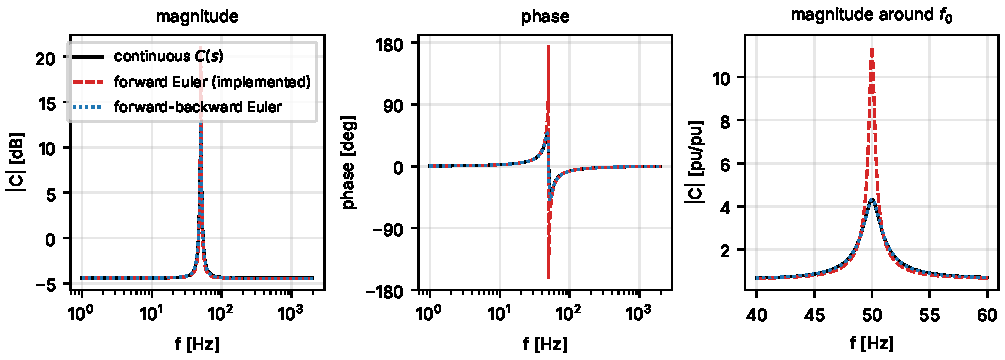
\includegraphics[width=\textwidth]{figures/res_pi_bode.pdf}
	\caption{Frequency response of the resonant PI, $k\ped{p} = 0.6$, $k\ped{i} = \SI{35}{\per\second}$, $\delta = 0.015$: continuous $C(s)$, the forward Euler implementation $C\ped{d}(z)$ of the code and the forward-backward Euler variant of Section~\ref{sec:rpi_alt}. Right: the peak at $f\ped{0}$, $4.3$ in continuous time and $11.4$ with forward Euler. Script \code{afe\_uvw\_ctrl\_figures.py}.}
	\label{fig:bode}
\end{figure}

\begin{figure}[H]
	\centering
	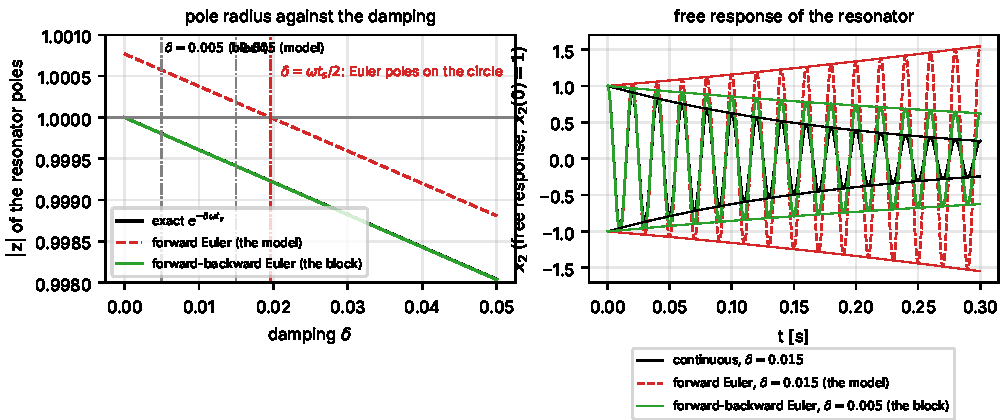
\includegraphics[width=\textwidth]{figures/res_pi_poles.pdf}
	\caption{Left: radius of the resonator poles against the damping $\delta$ for the exact mapping, the forward Euler of the code and the forward-backward Euler variant (the last two curves coincide with the exact one at this scale); the forward Euler poles are outside the unit circle for $\delta < \omega t\ped{s}/2 = 0.0196$. Right: free response of the resonator state $x_2$ from $x_2(0) = 1$: the continuous resonator decays, the forward Euler one grows by \SI{3}{\percent} per period.}
	\label{fig:poles}
\end{figure}

\subsection{What it means for the current loop}
\label{sec:rpi_loop}

A growing resonator does not make the loop unstable by itself: the poles of the closed loop are what counts, and the loop gain at \SI{50}{\hertz} moves them inside the circle. To show it with numbers, the loop is closed on the plant of the test bench of the package: three RL branches between the converter and the grid in pu, $x\ped{l} = 0.1$ (reactance at $f\ped{0}$) and $r = 0.01$, integrated exactly over one step,
\begin{equation}
	P(z) = \frac{K}{z - e\ped{p}}, \qquad e\ped{p} = e^{-r\omega t\ped{s}/x\ped{l}}, \quad K = \frac{1 - e\ped{p}}{r}, \qquad L(z) = C\ped{d}(z)\, z^{-1}\, P(z),
	\label{eq:loop}
\end{equation}
where $z^{-1}$ is the one-step output delay of the block (Section~\ref{sec:limiter}). The plant of the model (\SI{690}{\volt}, \SI{250}{\kilo\watt}, \SI{500}{\micro\henry}: $x\ped{l} = 0.092$ pu, $r = 0.0023$ pu) gives almost the same numbers. The results of the companion script:
\begin{center}
	\footnotesize
	\begin{tabular}{@{} l c c c c @{}}
		\toprule
		plant, resonator & crossover & phase margin & largest closed-loop $|z|$ & $|S|$ at \SI{50}{\hertz} \\
		\midrule
		bench, forward Euler (the code) & \SI{300}{\hertz} & \ang{68.9} & $0.99656$ & $0.0088$ (\SI{-41.1}{\decibel}) \\
		bench, forward-backward Euler & \SI{300}{\hertz} & \ang{68.9} & $0.99576$ & $0.0233$ (\SI{-32.7}{\decibel}) \\
		model \SI{690}{\volt}, forward Euler (the code) & \SI{327}{\hertz} & \ang{66.5} & $0.99651$ & $0.0080$ (\SI{-41.9}{\decibel}) \\
		model \SI{690}{\volt}, forward-backward Euler & \SI{327}{\hertz} & \ang{66.5} & $0.99571$ & $0.0213$ (\SI{-33.4}{\decibel}) \\
		\bottomrule
	\end{tabular}
\end{center}
The closed loop is stable with a good margin; the crossover (about \SI{300}{\hertz}, set by $k\ped{p}\omega\ped{nom}/x\ped{l}$) and the margin do not depend on the resonator, which is small away from \SI{50}{\hertz}. The resonant poles of the closed loop sit at $|z| = 0.9966$ (a time constant of \SI{36}{\milli\second}) and the sensitivity at \SI{50}{\hertz} is \SI{0.9}{\percent}: a \SI{50}{\hertz} disturbance (the grid voltage, when it is not fed forward by the modulator) is attenuated by \SI{41}{\decibel}, and the steady-state tracking error of a \SI{50}{\hertz} reference is below \SI{1}{\percent} of its amplitude. This is in fact \emph{better} than what the continuous design with $\delta = 0.015$ would give (\SI{2.3}{\percent}, the forward-backward row), because the implemented resonator has more gain at the grid frequency. The test bench confirms the order of magnitude: the stack current reaches its \SI{-0.85}{pu} reference within \num{6e-3} pu (Section~\ref{sec:checks}).

\begin{figure}[H]
	\centering
	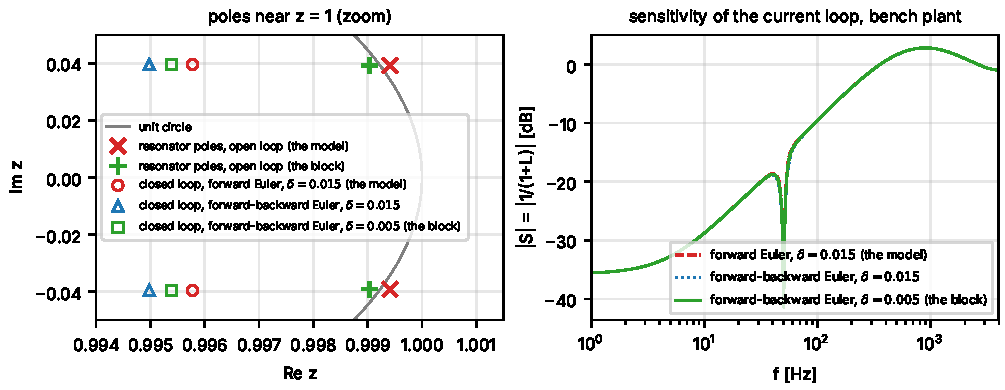
\includegraphics[width=\textwidth]{figures/res_pi_closed_loop.pdf}
	\caption{Per-phase current loop on the bench plant ($x\ped{l} = 0.1$, $r = 0.01$, one step of delay). Left: the open-loop resonator poles of the code (on the circle at this scale, radius $1.000182$) and the closed-loop poles with the forward Euler and the forward-backward resonator; the loop pulls the resonant pair inside the circle. Right: sensitivity $|S| = |1/(1+L)|$; the notch at \SI{50}{\hertz} is \SI{41}{\decibel} deep with the implemented resonator.}
	\label{fig:closed}
\end{figure}

Two consequences are worth keeping in mind:
\begin{itemize}[nosep]
	\item the stability of the resonant mode depends on the loop gain at \SI{50}{\hertz}. When the vector limiter of Section~\ref{sec:limiter} divides the output by \code{scale}, the loop gain drops by the same factor: with the bench plant the largest closed-loop radius grows from $0.99656$ (scale 1) to $0.99807$ (scale 5) and $0.99927$ (scale 10, the largest allowed), still inside the circle, but with a mode that decays about five times more slowly;
	\item the resonator states have no anti-windup: while the limiter is active, or while the modulator is disabled, $x_1$ and $x_2$ keep integrating with their own growing dynamics. The state of a locked loop (gates off) grows by \SI{3}{\percent} per period, so a long time with the gates off and a non-zero current error should be avoided, or the states should be reset (the block has no reset input: the subsystem can be re-initialized, or a reset can be added like the one of \code{frt\_vde4110}).
\end{itemize}

\subsection{A variant with the poles on the circle (not implemented)}
\label{sec:rpi_alt}

The usual remedy \cite{yepes2010} is to discretize the two integrators differently: forward Euler on the first and backward Euler on the second, that is, to use the \emph{updated} $x_1$ in the update of $x_2$:
\begin{equation}
	x_1^{+} = x_1 + t\ped{s}\, x_2, \qquad x_2^{+} = x_2 + t\ped{s}\left(-\omega^2 x_1^{+} - 2\delta\omega\, x_2 + k\ped{i}\, e\right),
	\label{eq:fb}
\end{equation}
one changed line in the code (\code{x\_res(1,:)} computed first and used in the second update). The characteristic polynomial becomes $z^2 - (2 - \omega^2 t\ped{s}^2 - 2\delta\omega t\ped{s})\, z + 1 - 2\delta\omega t\ped{s}$, so $|z\ped{res}| = \sqrt{1 - 2\delta\omega t\ped{s}}$: exactly on the unit circle for $\delta = 0$ and inside for any $\delta > 0$, with the resonance at \SI{50.012}{\hertz} and the peak gain $4.31$ of the continuous design (Figures~\ref{fig:bode} and \ref{fig:poles}). Tustin with pre-warping at $\omega$ gives the same result with more arithmetic. The variant is \emph{not} in the code, because the blocks reproduce the model and the gains of the model were tuned with the forward Euler resonator: changing the discretization alone would cut the gain at \SI{50}{\hertz} from $11.4$ to $4.3$ and the depth of the notch from \SI{41}{\decibel} to \SI{33}{\decibel}. If the variant is adopted, $\delta$ should be lowered to about $0.005$ to keep the present gain at the grid frequency ($k\ped{i}/(2\delta\omega) = 10.8$ gives $\delta = 0.0052$), or $\delta = 0$ can be used, now safely, for zero steady-state error.

\subsection{Vector limiter, transformation to $\alpha\beta$ and output delay}
\label{sec:limiter}

The three outputs $d\ped{abc}$ of the resonant PIs are divided by one common factor,
\begin{equation}
	\mathrm{scale} = \sat\!\big(|u_{\alpha\beta}(k-1)|,\ \code{mag\_lim},\ \code{mag\_scale\_max}\big), \qquad d\ped{abc} \leftarrow d\ped{abc}/\mathrm{scale},
	\label{eq:scale}
\end{equation}
where $|u_{\alpha\beta}(k-1)|$ is the length of the $\alpha\beta$ output vector of the previous step. With \code{mag\_lim} = 1 and \code{mag\_scale\_max} = 10 the factor is 1 as long as the voltage vector is inside the unit circle (the linear range of the modulator) and grows up to 10 when the controller asks for more: the vector is scaled, not clipped per phase, so its direction is kept. This is the \code{antiwind\_up} subsystem of the model. It acts one step late (it reads the previous output) and, as said above, it does not touch the resonator states.

The scaled outputs are transformed to $\alpha\beta$ with \eqref{eq:clarke}, which drops their zero sequence (the three resonant PIs are independent and their outputs need not sum to zero; the zero sequence of the voltage is set by the next loop instead). The result is delivered one step late when \code{out\_delay} is 1, as the Unit Delay blocks of the model do: the previous $u_{\alpha\beta}$ is output and the new one stored. The delay is part of the loop analysis of Section~\ref{sec:rpi_loop}; \code{out\_delay} = 0 removes it, for a model whose modulator already accounts for the computation delay.

\subsection{Zero-sequence current loop}
\label{sec:zseq}

The third component of the output, $u_\gamma$, is set by a PI with clamped integrator \eqref{eq:pi_clamped} on the zero-sequence current,
\begin{equation}
	i\ped{z} = \tfrac{1}{3}\left(i\ped{s,a} + i\ped{s,b} + i\ped{s,c}\right), \qquad e\ped{z} = \code{iz\_ref} - i\ped{z}, \qquad u_\gamma = \sat\!\big(k\ped{p,z} e\ped{z} + u\ped{i,z},\ \pm\code{u\_z\_lim}\big),
	\label{eq:zseq}
\end{equation}
with $k\ped{p,z} = 0.5$, $k\ped{i,z} = \SI{18}{\per\second}$, the limit \SI{1}{pu} and the reference 0. It cancels a common-mode current of the stack, for instance the one driven by a DC offset of the grid branches or by an asymmetry of the modulation. In the test bench a \SI{0.02}{pu} DC offset in the branch voltages is cancelled to \num{7e-13} pu.

\subsection{Log output}

\code{is\_xe} = [$\xi$; $\eta$] is the measured stack current in the positive frame (Clarke and rotation by $+\theta$), the \code{id\_xi\_pu}, \code{id\_eta\_pu} signals of the model, for the scopes. It is not used by the control.

% =============================================================
\section{Islanding detector (\code{islanding\_detector})}
\label{sec:island}

This block is new: the model had a subsystem that only measured the 7th harmonic of the grid voltage. Inputs: \code{ug\_ab} (from Section~\ref{sec:vseq}), \code{theta}, \code{omega\_pu}, \code{enable}. The detector is \emph{passive}: it watches what the voltage at the point of connection does when the grid is lost and the converter keeps feeding the local load, and it trips when one of six criteria holds for its whole on-delay (Table~\ref{tab:island}).

\paragraph{Measurements.} The fundamental and two harmonics are measured by turning $\alpha\beta$ with a multiple of the PLL angle and averaging over one grid period (the same moving average \eqref{eq:mavg} with $k\ped{avg}$ = \code{h\_avg\_order} = 1, which removes every other harmonic):
\begin{equation}
	\begin{aligned}
		\text{fundamental, positive frame:}\quad & \alpha c_1 + \beta s_1, \quad -\alpha s_1 + \beta c_1, \\
		\text{5th harmonic, negative frame:}\quad & \alpha c_5 - \beta s_5, \quad \alpha s_5 + \beta c_5, \\
		\text{7th harmonic, positive frame:}\quad & \alpha c_7 + \beta s_7, \quad -\alpha s_7 + \beta c_7,
	\end{aligned}
	\qquad c_h = \cos h\theta,\ s_h = \sin h\theta,
	\label{eq:harm}
\end{equation}
and $u_1$, $u_5$, $u_7$ are the lengths of the three averaged pairs. The harmonic criterion is the ratio $h = \sqrt{u_5^2 + u_7^2}\,/\max(u_1, u\ped{valid})$, with $u\ped{valid}$ = \code{u\_valid}: the 5th and the 7th are the harmonics that an inverter with dead time or a non-linear local load produces most, and they rise when the stiff grid is gone. The frequency is the PLL pulsation through a first-order low pass with time constant \code{tau\_f} (\SI{20}{\milli\second}), $f\ped{lpf} \leftarrow f\ped{lpf} + \frac{t\ped{s}}{\tau\ped{f} + t\ped{s}}(\omega\ped{pu} - f\ped{lpf})$, in pu; the ROCOF is the rate state of a double-integrator observer \eqref{eq:obs} on $\omega\ped{pu}$ with poles at $[-20,\ -80]$ \si{\radian\per\second} ($k_x = \SI{99.6}{\per\second}$, $k_v = \SI{1590}{\per\second\squared}$), scaled to \si{\hertz\per\second}.

\begin{table}[H]
	\centering
	\footnotesize
	\caption{Criteria of the islanding detector with the default thresholds (the network protection values of VDE-AR-N 4105 / 4110 \cite{vde4105,vde4110}, plus ROCOF and harmonics). Each criterion has its bit in \code{crit}.}
	\label{tab:island}
	\rowcolors{2}{tableShade}{white}
	\begin{tabular}{@{} c l l l c @{}}
		\toprule
		\textbf{bit} & \textbf{criterion} & \textbf{condition} & \textbf{on-delay} & \textbf{needs $u_1 \ge$ \code{u\_valid}} \\
		\midrule
		1 & under-voltage & $u_1 <$ \code{u\_min} = \SI{0.8}{pu} & \code{t\_trip\_u\_min} = \SI{2.7}{\second} & no \\
		2 & over-voltage & $u_1 >$ \code{u\_max} = \SI{1.15}{pu} & \code{t\_trip\_u\_max} = \SI{0.1}{\second} & no \\
		4 & under-frequency & $f\ped{lpf} <$ \code{f\_min} = \SI{47.5}{\hertz} & \code{t\_trip\_f} = \SI{0.1}{\second} & yes \\
		8 & over-frequency & $f\ped{lpf} >$ \code{f\_max} = \SI{51.5}{\hertz} & \code{t\_trip\_f} = \SI{0.1}{\second} & yes \\
		16 & ROCOF & $|\mathrm{d}f/\mathrm{d}t| >$ \code{rocof\_max} = \SI{2.5}{\hertz\per\second} & \code{t\_trip\_rocof} = \SI{0.1}{\second} & yes \\
		32 & harmonics & $h >$ \code{h\_max} = $0.1$ & \code{t\_trip\_h} = \SI{0.1}{\second} & yes \\
		\bottomrule
	\end{tabular}
	\rowcolors{1}{white}{white}
\end{table}

\paragraph{Logic.} A timer per criterion counts the time during which its condition holds and is reset when it does not; the bit is set when the timer reaches the on-delay. The frequency, ROCOF and harmonic criteria are blocked while $u_1 <$ \code{u\_valid} (\SI{0.5}{pu}): a PLL in a deep voltage dip is not a frequency meter, and a grid fault is the business of the FRT block, not of this one. The detector is armed when \code{enable} is high and \code{t\_enable} (\SI{0.1}{\second}) has passed; with \code{latch} = 1 the output \code{island} stays 1 from the first trip until \code{enable} goes to 0, otherwise it follows the criteria. The log gives $u_1$, $u_5$, $u_7$, $h$, $f\ped{lpf}$, the ROCOF, the longest running timer and the time since the detection.

\paragraph{Limits.} When the local load takes exactly the active and the reactive power of the converter, voltage and frequency do not move after the loss of the grid and only the harmonics can tell (the non-detection zone of every passive method). The slow under-voltage stage (\SI{0.8}{pu} for \SI{2.7}{\second}) is what lets the converter ride through a grid fault without an islanding trip: in the test bench the dip of \SI{150}{\milli\second} does not trip the detector, while a frequency ramp of \SI{6}{\hertz\per\second} (the grid lost with a surplus of active power) trips the ROCOF criterion \SI{0.14}{\second} after its start (Figure~\ref{fig:bench}). In the model the block is in the library but not yet wired (Section~\ref{sec:open}).

% =============================================================
\section{Parameter structure and the model init}
\label{sec:params}

All five blocks read the same structure \code{p}: the common fields at the top level and one sub-structure per block (Table~\ref{tab:params}). The file \code{afe\_uvw\_ctrl\_param\_example.m} of the package builds it with the numbers of the model, \code{p = afe\_uvw\_ctrl\_param\_example(ts, f\_nom)}, and computes the observer gains with \eqref{eq:obs_gains}. In the model the section ``AFE control in uvw'' of \code{init\_model.m} builds \code{param.afe.uvw} field by field from the existing objects of the init (\code{param.afe.ctrl} from the class \code{ctrl\_afe\_setup}, \code{param.frt.data}, \code{param.ctrl}, \code{param.glb\_time}, \code{param.grid}), so that a change of a gain in the init reaches the blocks; the section comes after ``Control settings common to all modules'' because it reads \code{param.ctrl}. The last column of the table says where each number comes from in the model.

{\footnotesize
\setlength{\tabcolsep}{4pt}
\setlength{\LTcapwidth}{\textwidth}
\rowcolors{2}{tableShade}{white}
\begin{longtable}{@{} p{3.2cm} p{5.4cm} p{1.7cm} p{4.5cm} @{}}
	\caption{The parameter structure \code{p} (\code{param.afe.uvw} in the model): fields, meaning, values of the model and their source in \code{init\_model.m} (\code{c} = \code{param.afe.ctrl}).}
	\label{tab:params} \\
	\toprule
	\textbf{field} & \textbf{meaning} & \textbf{value} & \textbf{source in the model} \\
	\midrule
	\endfirsthead
	\toprule
	\textbf{field} & \textbf{meaning} & \textbf{value} & \textbf{source in the model} \\
	\midrule
	\endhead
	\bottomrule
	\endfoot
	\bottomrule
	\endlastfoot
	\multicolumn{4}{@{}l}{\textbf{common}} \\
	\code{ts} & control period [s], integration step of all blocks & \num{125e-6} & \code{param.glb\_time.ts\_afe} \\
	\code{omega\_nom} & nominal grid pulsation [rad/s], base of \code{omega\_pu} & $2\pi\,50$ & \code{param.grid.emu.}\newline\code{omega\_grid\_nom} \\
	\multicolumn{4}{@{}l}{\textbf{vseq} (grid voltage sequences) and \textbf{iseq} (grid current sequences), same four fields} \\
	\code{avg\_order} & window = grid period / \code{avg\_order} (2: half period) & 2 & \code{param.ctrl.mavarage\_filter\_}\newline\code{frequency\_base\_order} \\
	\code{omega\_pu\_min}, \code{\_max} & limits of the measured pulsation used for the window [pu] & 0.1, 2 & constants of the model's saturation \\
	\code{t\_enable} & averages are zero before this time [s] & 0.025 & \code{param.ctrl.}\newline\code{dmavg\_filter\_enable\_time} \\
	\multicolumn{4}{@{}l}{\textbf{iseq}, the three PIs} \\
	\code{kp\_pos}, \code{ki\_pos} & PI of the positive-sequence $\eta$ grid current, [--], [1/s] & 0.25, 35 & \code{c.kp\_rc\_pos\_grid}, \code{c.ki\_rc\_pos\_grid} \\
	\code{kp\_neg}, \code{ki\_neg} & PI of the negative-sequence $\xi$ and $\eta$ grid currents & 0.25, 35 & \code{c.kp\_rc\_neg\_grid}, \code{c.ki\_rc\_neg\_grid} \\
	\code{lim\_pos\_eta} & limit of the stack current reference pos\_eta [pu] & 1.0 & \code{c.ieta\_pos\_ref\_lim} \\
	\code{lim\_neg\_xi} & limit of neg\_xi [pu] (the model uses the positive limit) & 1.0 & \code{c.ieta\_pos\_ref\_lim} \\
	\code{lim\_neg\_eta} & limit of neg\_eta [pu] & 0.5 & \code{c.ieta\_neg\_ref\_lim} \\
	\code{err\_sign} & $-1$: grid current measured towards the converter & $-1$ & the gain $-1$ of the model's diagram \\
	\multicolumn{4}{@{}l}{\textbf{frt}} \\
	\code{obs\_kx}, \code{obs\_kv} & gains of the voltage-rate observers [1/s], [1/s$^2$] & 156.0, 3909 & \code{c.vr\_obs.kx}, \code{c.vr\_obs.kv}\newline(poles $[-0.1, -0.4]\,\omega$) \\
	\code{t\_obs\_release} & observers held at zero before this time [s] & 0.025 & \code{time\_release} of the model \\
	\code{v\_pos\_low}, \code{v\_pos\_high} & band of the positive sequence [pu] & 0.85, 1.15 & \code{LVRT\_VPOS\_TH\_LOW},\newline\code{LVRT\_VPOS\_TH\_HIGH} \\
	\code{v\_hyst} & band narrowing to leave the fault [pu] & 0.1 & \code{LVRT\_SEQ\_DETECTION\_HYST} \\
	\code{v\_neg\_max} & negative sequence above this is a fault [pu] & 0.1 & \code{LVRT\_VNEG\_TH} \\
	\code{v\_pos\_dot\_max},\newline\code{v\_neg\_dot\_max} & voltage rate needed for a detection [pu/s] & 2, 2 & \code{LVRT\_VPOS\_DOT\_TH}, \code{LVRT\_VNEG\_DOT\_TH} \\
	\code{t\_rearm} & idle time before a new detection [s] & 0.125 & 1000 samples of the model \\
	\code{t\_hold\_max} & fault longer than this: EXCEEDED [s] & 7.625 & 61000 samples of the model \\
	\code{pwrlim\_v\_pos},\newline\code{pwrlim\_v\_neg} & power limitation when pos\_xi below / $|v\ped{neg}|$ above [pu] & 0.8, 0.1 & \code{LVRT\_VPOS\_PWRLIM\_TH},\newline\code{LVRT\_VNEG\_PWRLIM\_TH} \\
	\code{pwrlim\_hyst} & release when pos\_xi $>$ \code{pwrlim\_v\_pos} + this [pu] & 0.1 & the model's diagram \\
	\code{pwrlim\_v\_neg\_release} & \ldots and $|v\ped{neg}|$ below this [pu] & 0.7 & the model's diagram (see open points) \\
	\code{reddyn\_enabled} & reduced dynamic support on/off & 0 & constant 0 of the model \\
	\code{reddyn\_v\_pos},\newline\code{reddyn\_v\_neg} & thresholds of the reduced support [pu] & 0.7, 0.2 & \code{LVRT\_VPOS\_RED\_DYN\_TH},\newline\code{LVRT\_VNEG\_RED\_DYN\_TH} \\
	\code{k\_frt\_ref} & reactive current per voltage change [pu/pu] & 2 & \code{param.frt.data.k\_frt\_ref} \\
	\code{t\_avg\_prefault} & window of the pre-fault averages [s] & 0.5 & \code{avg\_flt\_500ms} of the model \\
	\code{t\_avg\_start} & the pre-fault averages start here [s] & 0.05 & new (the model started at 0) \\
	\code{lim\_pos\_eta},\newline\code{lim\_neg\_xi}, \code{lim\_neg\_eta} & limits of the grid current references [pu] & 1.0, 0.5, 0.5 & \code{c.i\_grid\_pos\_eta\_lim},\newline\code{c.i\_grid\_neg\_xi\_lim},\newline\code{c.i\_grid\_neg\_eta\_lim} \\
	\code{lim\_*\_red} & the same with reduced dynamic support [pu] & 0.1 & \code{c.i\_grid\_*\_red\_lim} \\
	\code{f\_lpf\_ref} & low pass of the references [Hz] & 161 & \code{g0\_161Hz} of the model \\
	\multicolumn{4}{@{}l}{\textbf{ictrl}} \\
	\code{kp}, \code{ki} & resonant PI: proportional gain [--] and resonant gain [1/s] & 0.6, 35 & \code{c.res\_pi.kp\_rpi}, \code{c.res\_pi.ki\_rpi}\newline(LVRT setting of the init; class defaults 0.2, 45) \\
	\code{delta\_res} & damping of the resonator & 0.015 & \code{c.res\_pi.delta\_res} \\
	\code{omega\_res} & resonance pulsation [rad/s] & $2\pi\,50$ & \code{c.omega\_base} \\
	\code{mag\_lim}, \code{mag\_scale\_max} & vector limiter: length above which the output is scaled, largest factor & 1, 10 & constants of \code{antiwind\_up} \\
	\code{out\_delay} & 1: $\alpha\beta$ output one step late (Unit Delays of the model) & 1 & -- \\
	\code{kp\_z}, \code{ki\_z} & zero-sequence current PI [--], [1/s] & 0.5, 18 & \code{c.kp\_is\_z}, \code{c.ki\_is\_z} \\
	\code{u\_z\_lim}, \code{iz\_ref} & limit of $u_\gamma$ [pu], zero-sequence reference [pu] & 1, 0 & constants of the model \\
	\multicolumn{4}{@{}l}{\textbf{island} (new block: all values are defaults of the library)} \\
	\code{h\_avg\_order} & harmonic averaging window = grid period / this & 1 & \\
	\code{omega\_pu\_min}, \code{\_max} & limits of the measured pulsation for the window [pu] & 0.5, 1.5 & \\
	\code{t\_enable} & no detection before this time [s] & 0.1 & \\
	\code{tau\_f} & low pass of the frequency [s] & 0.02 & \\
	\code{obs\_poles},\newline\code{obs\_kx}, \code{obs\_kv} & ROCOF observer: poles [rad/s] and gains [1/s], [1/s$^2$] & $[-20, -80]$,\newline 99.6, 1590 & the init computes the gains with \code{acker} \\
	\code{u\_valid} & frequency and harmonic criteria only above this voltage [pu] & 0.5 & \\
	\code{u\_min}, \code{t\_trip\_u\_min} & under-voltage [pu], [s] & 0.8, 2.7 & VDE-AR-N 4105 / 4110 \\
	\code{u\_max}, \code{t\_trip\_u\_max} & over-voltage [pu], [s] & 1.15, 0.1 & VDE-AR-N 4105 / 4110 \\
	\code{f\_min}, \code{f\_max}, \code{t\_trip\_f} & frequency band [pu], delay [s] & 47.5/50, 51.5/50, 0.1 & VDE-AR-N 4105 / 4110 \\
	\code{rocof\_max}, \code{t\_trip\_rocof} & ROCOF [Hz/s], delay [s] & 2.5, 0.1 & \\
	\code{h\_max}, \code{t\_trip\_h} & harmonic ratio [--], delay [s] & 0.1, 0.1 & \\
	\code{latch} & 1: output stays 1 until \code{enable} goes to 0 & 1 & \\
\end{longtable}
\rowcolors{1}{white}{white}
}

% =============================================================
\section{How the code was checked}
\label{sec:checks}

\paragraph{Python twin of the model's diagrams.} The script \code{tools/check\_afe\_uvw\_ctrl.py} of the package holds a twin, in Python and without MATLAB, of the Simulink diagrams that were replaced (\code{dmavgflt\_process}, \code{LVRT\_detector}, \code{linear\_double\_integrator\_observer}, \code{avg\_flt}, \code{u\_161Hz\_flt}, the resonant PIs, \code{antiwind\_up}, \code{zero\_sequence\_current\_ctrl}, written block by block from the \code{.slx} and from the library sources) and runs it together with the five functions (in GNU Octave) on the same inputs for \SI{1.2}{\second}: a \SI{50.2}{\hertz} grid with \SI{2}{\percent} 7th and \SI{1.5}{\percent} 5th harmonic, a dip to \SI{0.55}{pu} with \SI{0.25}{pu} negative sequence at 0.75--\SI{0.90}{\second}, steps of the grid current and of the references. The comparison is made block by block (the twin reads the signals of the new code at the block borders, so that each block sees the same inputs): the transformations agree to \num{4e-16}, the observers to \num{7e-14}, the PIs of the reactive loops to \num{4e-14}, the current controller (\code{u\_abg}, \code{i\_abc\_ref}) to \num{4e-13}; the sequence averages differ by \num{2e-4} in steady state and \num{3e-3} at the edges of the dip (a different moving average, Section~\ref{sec:differences}), the FRT references by \num{5e-4} (pre-fault average one sample apart), and the two implementations detect the fault at the same samples (\SI{0.75488}{\second}, \SI{0.90813}{\second}). Figure~\ref{fig:check} shows the chain run.

\begin{figure}[H]
	\centering
	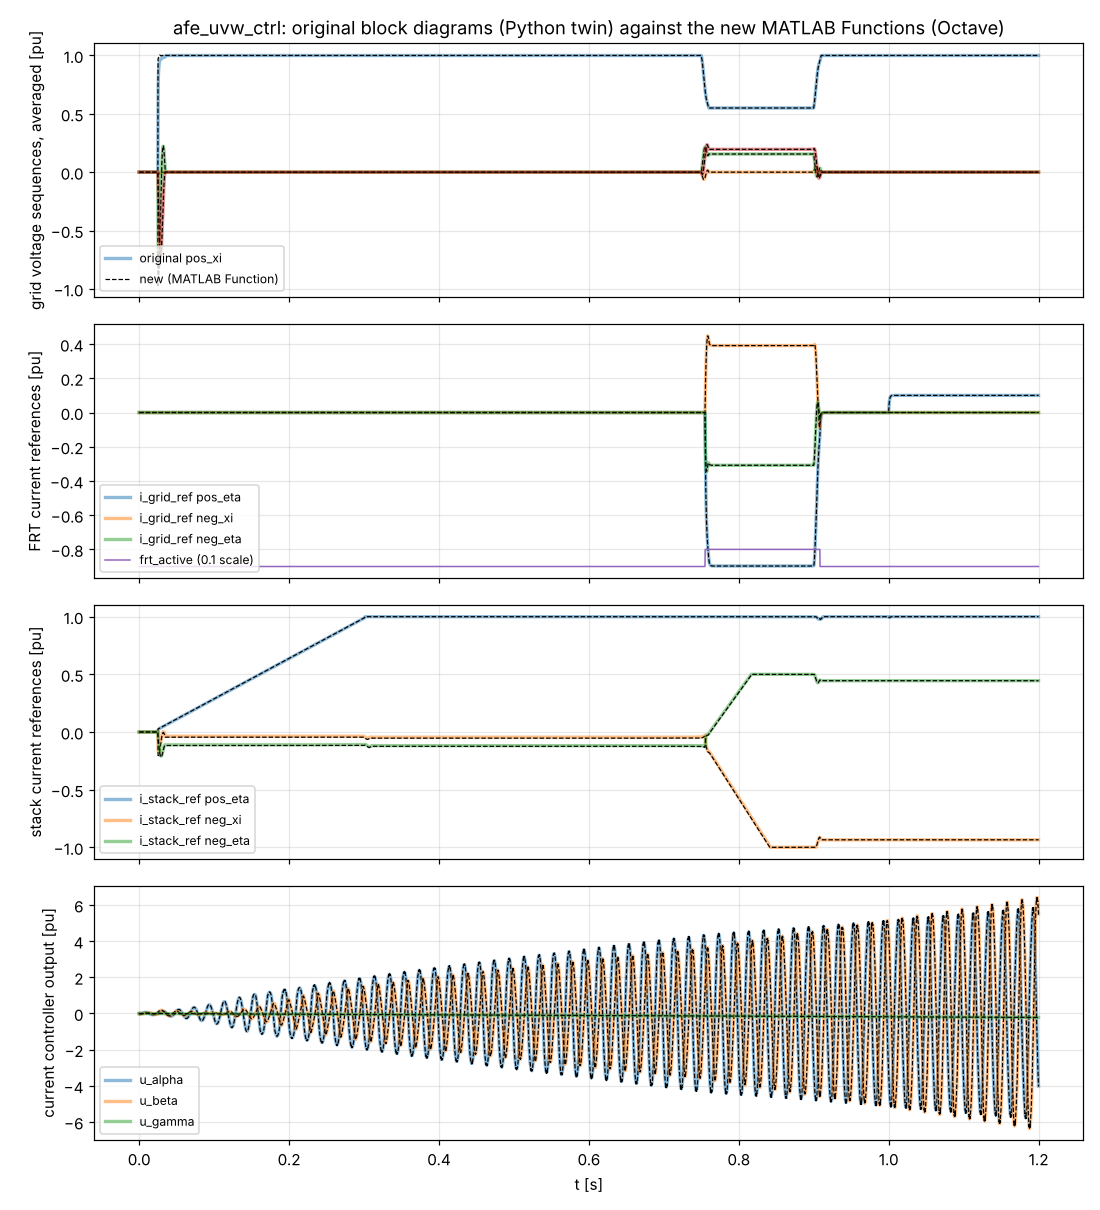
\includegraphics[width=0.8\textwidth]{figures/check_afe_uvw_ctrl.png}
	\caption{The Python twin of the original block diagrams (solid) against the five MATLAB Functions run in GNU Octave (dashed), each implementation on its own signals, open loop: averaged voltage sequences, FRT references, stack current references of the reactive loops and the output of the current controller (which grows because the loop is open: the resonators integrate the error of a current that never comes).}
	\label{fig:check}
\end{figure}

\paragraph{The test bench in a loop.} \code{test/afe\_uvw\_ctrl\_test\_loop.m} runs the five functions in a loop with a source (grid voltage with harmonics, PLL angle, references) and the RL plant of \eqref{eq:loop} behind a unit delay, \SI{1.6}{\second}; \code{afe\_uvw\_ctrl\_test\_run.m} runs the same scenario in the Simulink bench \code{test\_afe\_uvw\_ctrl.slx} and in the loop and prints 15 checks. In GNU Octave the 14 behaviour checks pass: fault detected \SI{5}{\milli\second} after the start of the dip and released \SI{8}{\milli\second} after its end, power limitation set, FRT reference \SI{-0.80}{pu} reached within \num{3e-3}, grid $\eta$ current on its reference within \num{5e-5} before the dip and within $0.02$ at the end of the dip, stack $\xi$ current on \SI{-0.85}{pu} within \num{6e-3}, zero-sequence current \num{7e-13}, islanding detected \SI{0.14}{\second} after the start of the \SI{6}{\hertz\per\second} ramp by the ROCOF criterion and not by the dip (Figure~\ref{fig:bench}). In MATLAB R2026b all 15 checks pass, the 15th being ``blocks = functions'': the Simulink bench and the loop give the same signals (difference 0).

\begin{figure}[H]
	\centering
	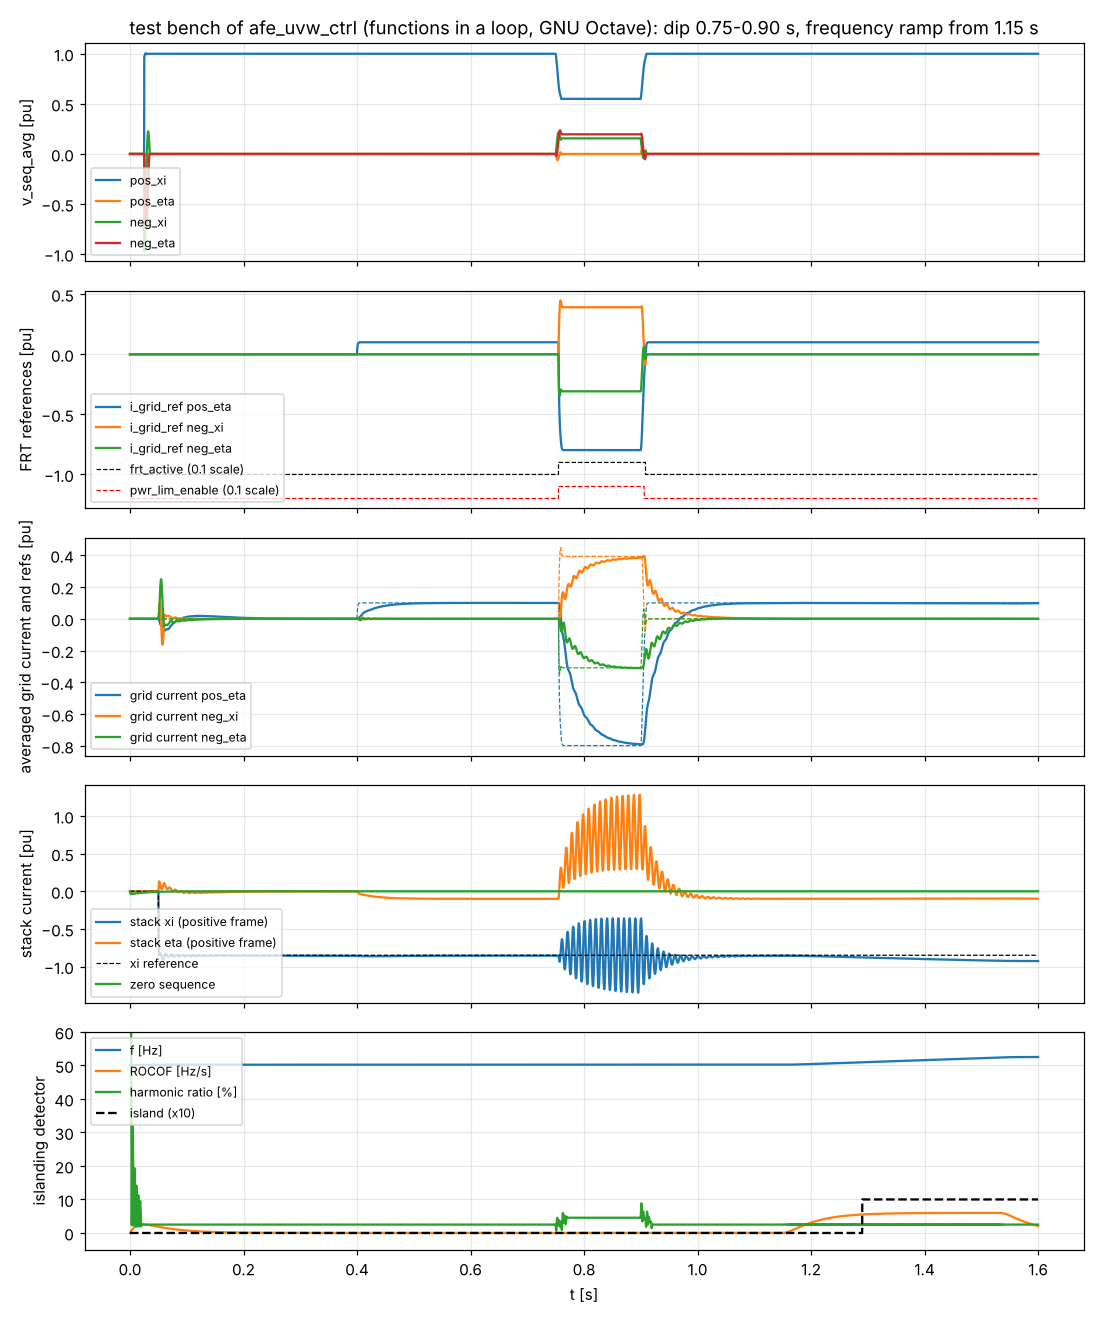
\includegraphics[width=0.8\textwidth]{figures/test_bench_loop.png}
	\caption{Test bench of the package run as a loop in GNU Octave: averaged voltage sequences, FRT references and flags, averaged grid current against its references, stack current in the positive frame with the zero sequence, and the islanding detector (frequency, ROCOF, harmonic ratio, trip). Dip at 0.75--\SI{0.90}{\second}, frequency ramp of \SI{6}{\hertz\per\second} from \SI{1.15}{\second}.}
	\label{fig:bench}
\end{figure}

\paragraph{In the model.} \code{afe\_rst\_ctrl.slx} of \code{afe\_uvw\_three\_phase} now uses the five blocks inside \code{afe\_control}, all with the mask parameter \code{param.afe.uvw} (Section~\ref{sec:params}); the model compiles with the explicit port sizes of the blocks (library PR \#35). The runs of the model with the new blocks belong to the model, not to this note.

% =============================================================
\section{Differences from the Simulink subsystems they replace}
\label{sec:differences}

\begin{itemize}[nosep]
	\item \textbf{Moving average.} \code{dmavgflt\_process} (the MATLAB port of the C \code{mavgflt}) averages the samples up to the previous one and starts from an implicit zero sample; \code{moving\_average\_frac} includes the present sample and is unbiased while the window fills up. Same steady-state value (within the $2\omega$ residual, \num{2e-4}), one sample of lead, no start-up transient.
	\item \textbf{Pre-fault averages of the FRT} start at \code{t\_avg\_start} (\SI{50}{\milli\second}) instead of 0: the model's average takes the zeros and the start-up transient of the sequence averages into its \SI{0.5}{\second} window, which puts an offset of about \num{1e-2} on the negative-sequence references of a fault in the first second.
	\item \textbf{\code{frt\_state} in the log} is the state after the update of the step (the model reported the state of the previous step); \code{frt\_active} and \code{pwr\_lim\_enable} have the same timing as the model.
	\item \textbf{Power-limitation release} on $|v\ped{neg}| < 0.7$, as in the model's diagram, where the threshold used is \code{LVRT\_VPOS\_PWRLIM\_TH} minus the hysteresis (probably a slip); the value is the parameter \code{pwrlim\_v\_neg\_release}.
	\item \textbf{Reduced dynamic support} is a parameter (default off) instead of the constant 0 of the model.
	\item \textbf{Islanding detector} is new; the model only measured the 7th harmonic.
	\item \textbf{Port sizes} of the MATLAB Functions are explicit (the model could not resolve the inherited sizes of \code{i\_abc\_ref}).
	\item The feed-forward of the grid voltage, the DC-link control, the PLL and the modulator are not part of these blocks, as they were not part of the replaced subsystems.
\end{itemize}

% =============================================================
\section{Open points}
\label{sec:open}

\begin{enumerate}[nosep]
	\item \textbf{Direction of the reactive current support.} With the $\eta$ axis of \eqref{eq:frames} (the usual $q$ axis) and the grid voltage on $+\xi$, a current measured \emph{into} the converter that leads the voltage by \ang{90} (capacitive, the support that VDE-AR-N 4110 asks for in an under-voltage) has a \emph{positive} $\eta$ component. The FRT rule \eqref{eq:frt_ref} gives a \emph{negative} $\eta$ reference in a dip, so the support is capacitive only if the grid current of the model is measured \emph{out of} the converter, towards the grid; with the grid current measured towards the converter (as the sign of the reactive loops suggests, Section~\ref{sec:qctrl}) it would be inductive. The code reproduces the model exactly here (the twin agrees to \num{4e-13}), so this is a check to make once on the model with the real plant: during a dip with \code{i\_react\_ref} = 0, the positive-sequence voltage at the connection point must rise with the support, not fall. If it falls, the sign of $k$ in \eqref{eq:frt_ref} (or of \code{k\_frt\_ref}) is the place to change it.
	\item \textbf{Forward Euler resonator.} The resonator of the current controller has its poles outside the unit circle for $\delta < \omega t\ped{s}/2$ (Section~\ref{sec:rpi_disc}); the loop is stable with the plant, but the controller alone grows, the resonant mode of the loop depends on the loop gain, and the states have no anti-windup. The variant of Section~\ref{sec:rpi_alt} (one line) puts the poles on or inside the circle; it changes the gain at \SI{50}{\hertz}, so $\delta$ would be re-tuned with it (about $0.005$ for the same gain, or 0 for zero steady-state error). A reset input for the states would help after a long time with the gates off.
	\item \textbf{Islanding detector not wired.} In \code{afe\_rst\_ctrl.slx} the block exists in the library but is not connected: its inputs would be \code{ug\_ab} of \code{grid\_voltage\_sequences}, the PLL angle, the limited pulsation and an enable (the settle time of the model), its output \code{island} a trip of the converter. With the thresholds of Table~\ref{tab:island} it does not trip on the FRT test dip.
	\item \textbf{Power-limitation release} on $|v\ped{neg}| < 0.7$ is almost no condition: a tighter value (e.g. $0.05$, with the same hysteresis idea as the positive sequence) would release the power limitation only when the unbalance is really gone.
	\item \textbf{\code{i\_stack\_ref} in the model} is built with a Bus Creator; the block expects a $3 \times 1$ vector (a Mux).
\end{enumerate}

% =============================================================
\section{Files}
\label{sec:files}

\begin{table}[H]
	\centering
	\footnotesize
	\caption{Files of the package and of this note.}
	\label{tab:files}
	\rowcolors{2}{tableShade}{white}
	\begin{tabularx}{\textwidth}{@{} l X @{}}
		\toprule
		\textbf{File} & \textbf{Content} \\
		\midrule
		\multicolumn{2}{@{}>{\raggedright\arraybackslash}p{\dimexpr\textwidth-2\tabcolsep\relax}@{}}{\textbf{folder \code{library/masked\_models/afe\_uvw\_ctrl/} of \code{pwr-control/library}}} \\
		\code{afe\_uvw\_ctrl.slx} & the library with the five masked MATLAB Function blocks \\
		\code{src/*.m} & the five functions, one file each, with their helper functions at the end (\code{moving\_average\_frac}, \code{pi\_clamped}, \code{moving\_sum\_push}) \\
		\code{afe\_uvw\_ctrl\_param\_example.m} & example parameter structure \code{p} with the numbers of the model and the observer gain formula \eqref{eq:obs_gains} \\
		\code{update\_afe\_uvw\_ctrl.m} & reloads the sources into the blocks of the library (MATLAB) \\
		\code{test/} & Simulink bench \code{test\_afe\_uvw\_ctrl.slx}, its source, plant and parameters, the loop version and the 15 checks \\
		\code{tools/make\_afe\_uvw\_ctrl.py}, \code{check\_afe\_uvw\_ctrl.py} & generator of the library and the bench without MATLAB; the check against the Python twin of the model's diagrams \\
		\code{README.md} & description of the blocks, parameters, checks and use in the model \\
		\midrule
		\multicolumn{2}{@{}>{\raggedright\arraybackslash}p{\dimexpr\textwidth-2\tabcolsep\relax}@{}}{\textbf{model \code{foundations\_of\_power\_electronics/afe\_uvw\_three\_phase/} of \code{pwr-control/modelization-and-control}}} \\
		\code{afe\_rst\_ctrl.slx}, \code{init\_model.m} & the model with the blocks inside \code{afe\_control}; the section ``AFE control in uvw'' of the init builds \code{param.afe.uvw} \\
		\midrule
		\multicolumn{2}{@{}>{\raggedright\arraybackslash}p{\dimexpr\textwidth-2\tabcolsep\relax}@{}}{\textbf{this note, \code{repos\_doc/afe\_uvw\_ctrl/} of \code{pwr-control/repositories-documentation}}} \\
		\code{afe\_uvw\_ctrl.tex}, \code{.pdf} & source and PDF \\
		\code{afe\_uvw\_ctrl\_figures.py} & the numbers of Section~\ref{sec:current} and Figures~\ref{fig:bode}--\ref{fig:closed} (numpy, matplotlib); writes \code{figures/afe\_uvw\_ctrl\_numbers.txt} \\
		\code{figures/} & the PDF figures of the script and the two PNG figures of the checks \\
		\bottomrule
	\end{tabularx}
	\rowcolors{1}{white}{white}
\end{table}

% =============================================================
\begin{thebibliography}{99}
	\bibitem{library_repo} pwr-control, \textit{library} repository, package \path{library/masked_models/afe_uvw_ctrl} (sources, README, tests), \url{https://github.com/pwr-control/library}.
	\bibitem{mc_repo} pwr-control, \textit{modelization-and-control} repository, model \path{foundations_of_power_electronics/afe_uvw_three_phase}, \url{https://github.com/pwr-control/modelization-and-control}.
	\bibitem{vde4110} VDE-AR-N 4110:2018-11, \textit{Technical requirements for the connection and operation of customer installations to the medium voltage network (TAR medium voltage)}, VDE FNN, 2018.
	\bibitem{vde4105} VDE-AR-N 4105:2018-11, \textit{Generators connected to the low-voltage distribution network}, VDE FNN, 2018.
	\bibitem{teodorescu2006} R.~Teodorescu, F.~Blaabjerg, M.~Liserre, and P.~C. Loh, ``Proportional-resonant controllers and filters for grid-connected voltage-source converters,'' \emph{IEE Proc. Electr. Power Appl.}, vol.~153, no.~5, pp.~750--762, Sept. 2006.
	\bibitem{yepes2010} A.~G. Yepes, F.~D. Freijedo, J.~Doval-Gandoy, O.~L\'opez, J.~Malvar, and P.~Fernandez-Comesa\~na, ``Effects of discretization methods on the performance of resonant controllers,'' \emph{IEEE Trans. Power Electron.}, vol.~25, no.~7, pp.~1692--1712, July 2010.
	\bibitem{teodorescu2011} R.~Teodorescu, M.~Liserre, and P.~Rodr\'iguez, \emph{Grid Converters for Photovoltaic and Wind Power Systems}. Wiley-IEEE Press, 2011.
	\bibitem{song1999} H.-S. Song and K.~Nam, ``Dual current control scheme for PWM converter under unbalanced input voltage conditions,'' \emph{IEEE Trans. Ind. Electron.}, vol.~46, no.~5, pp.~953--959, Oct. 1999.
	\bibitem{gfm_afe_note} D.~Bagnara, \textit{Grid-forming and grid-following AFE blocks: two-level bridge with LCL filter, description and user guide}, pwr-control technical note, Rev.~00, October 2026, \path{repos_doc/grid_forming_following_afe} of \url{https://github.com/pwr-control/repositories-documentation}.
\end{thebibliography}

\end{onehalfspace}
\end{document}
